\documentclass{beamer}
\usepackage{ulem}
\usepackage{tikz}
\usepackage{booktabs}
 \usepackage{graphicx,threeparttable,caption}
\usetikzlibrary{shapes,snakes}
\usepackage[beamer,customcolors]{hf-tikz}
\usepackage{nicematrix}
\usepackage{xcolor}
\usepackage{makecell}
\usepackage{array}
\usepackage{csquotes}
\usepackage{csquotes}
\usepackage{minted}
\captionsetup{labelformat=empty,labelsep=none}

\graphicspath{ {./png/} }

\usetikzlibrary{
    arrows,
    arrows.meta,
    shapes,
    positioning,
    shadows,
    trees,
    calc
}

\tikzset{%
    >={Latex[width=2mm,length=2mm]},
    % Specifications for style of nodes:
    plain/.style = {},
    base/.style = {
        plain,
        rectangle, rounded corners, draw=black,
        minimum width=1cm, minimum height=1cm,
        text centered, font=\sffamily\tiny\bfseries,
        fill=white, align=center
    },
    app/.style = {base, ellipse},
    data/.style = {base, fill=gray!30},
    action/.style = {base, circle, fill=red!30},
    note/.style = {app, fill=yellow},
    hl/.style={
    set fill color=red!80!black!40,
    set border color=red!80!black
    }
}


\AtBeginSection[]{
  \begin{frame}
  \vfill
  \centering
  \begin{beamercolorbox}[sep=8pt,center,shadow=true,rounded=true]{title}
    \usebeamerfont{title}\insertsectionhead\par%
  \end{beamercolorbox}
  \vfill
  \end{frame}
}
%\usecolortheme[orchid]{structure}
\usetheme[hideothersubsections]{PaloAlto}
\makeatletter
\patchcmd{\csq@bquote@i}{{#6}}{{\emph{#6}}}{}{}
\makeatother
%\usecolortheme{orchid}
%\usefonttheme{professionalfonts}
\newcommand{\soutthick}[1]{%
   \textcolor{red}{
   \renewcommand{\ULthickness}{1pt}%
      \sout{#1}%
   \renewcommand{\ULthickness}{.4pt}% Resetting to ulem default
   }
}
\newcommand{\centered}[1]{\begin{tabular}{l} #1 \end{tabular}}
\setbeamertemplate{section in toc}[square]
\setbeamertemplate{subsection in toc}[square]
\setbeamertemplate{secion in sidebar}[shaded]
\setbeamertemplate{items}[square]
\setbeamercovered{transparent} 

\title[]{Computational Social Science: An Introduction to Data Science}
\subtitle{Extracting existing data from external sources}
\author[]{Mikołaj Biesaga\\ \small{\color{blue}{\href{mailto:m.biesaga@uw.edu.pl}{m.biesaga@uw.edu.pl}}}}
\institute{
\includegraphics[width = 4 cm]{uw.png}}
\date{\today}
\begin{document}
\begin{frame}
   \titlepage
\end{frame}

\section{Examples}

%% \begin{frame}
%%     \frametitle{Twitter}
%%     \only<1>{
%%         \begin{figure}
%%             \centering
%%             
\includegraphics[width = .3\textwidth]{twitter_log.png}
%%         \end{figure}
%%     }
%%     \only<2>{
%%         \begin{figure}
%%             \centering
%%             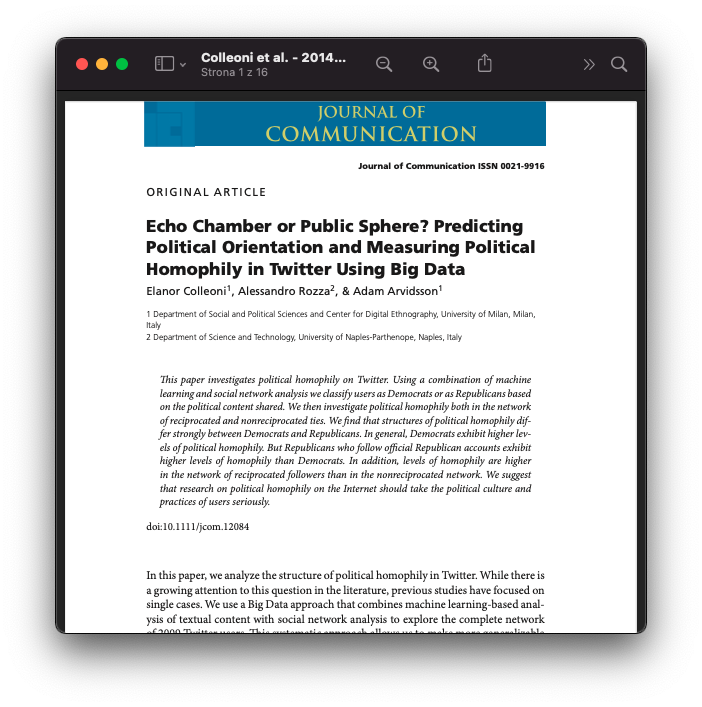
\includegraphics[width = \textwidth]{twitter1.png}
%%         \end{figure}
%%     }
%%     \only<3>{
%%         \begin{figure}
%%             \centering
%%             
\includegraphics[width = \textwidth]{twitter2.png}
%%         \end{figure}
%%     }
%%     
%% \end{frame}
\begin{frame}
    \frametitle{Reddit}
    \only<+>{
        \begin{figure}
            \centering
            
\includegraphics[width = .3\textwidth]{reddit_log.png}
        \end{figure}
    }
    \only<+>{
        \begin{figure}
            \centering
            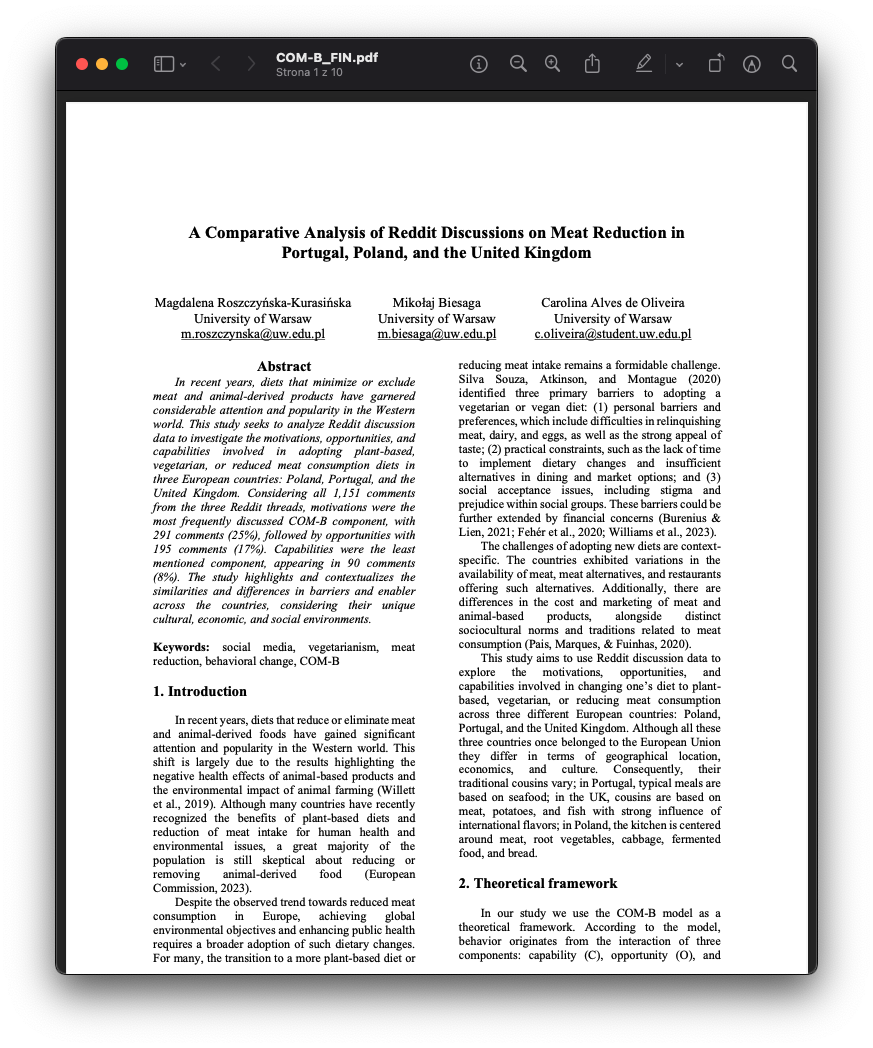
\includegraphics[width = \textwidth]{hicss.png}
        \end{figure}
    }
    \only<+>{
        \framesubtitle{(Roszczyńska-Kurasińska et al., 2025)}
        \begin{figure}
            \centering
            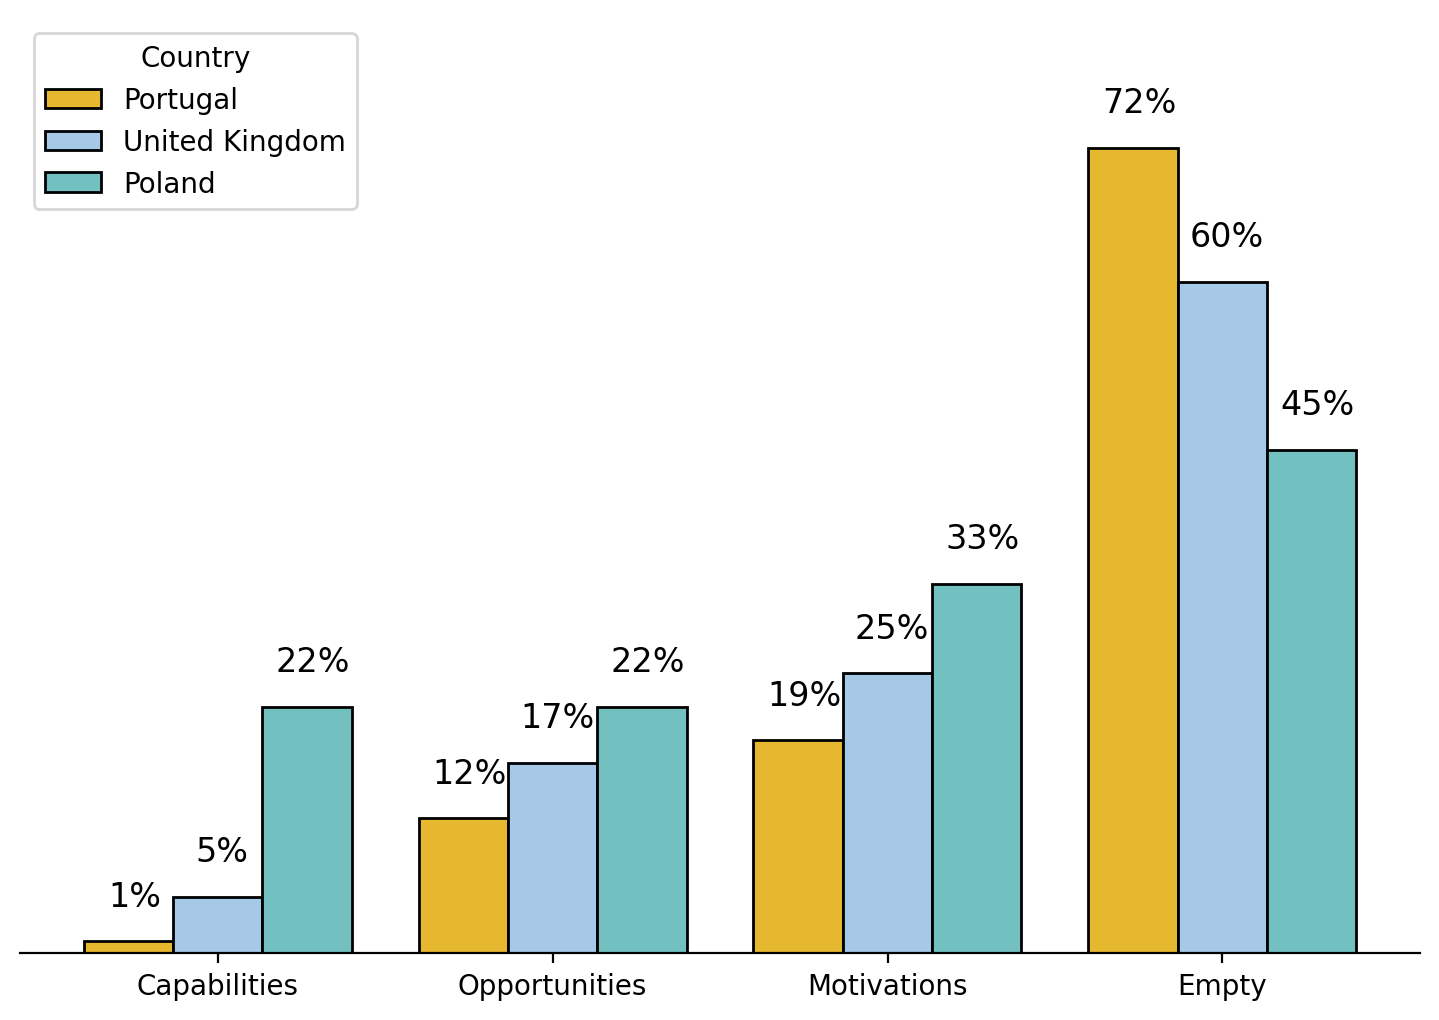
\includegraphics[width = \textwidth]{hicss-figure.png}
        \end{figure}

    }
    \only<+>{
        \begin{figure}
            \centering
            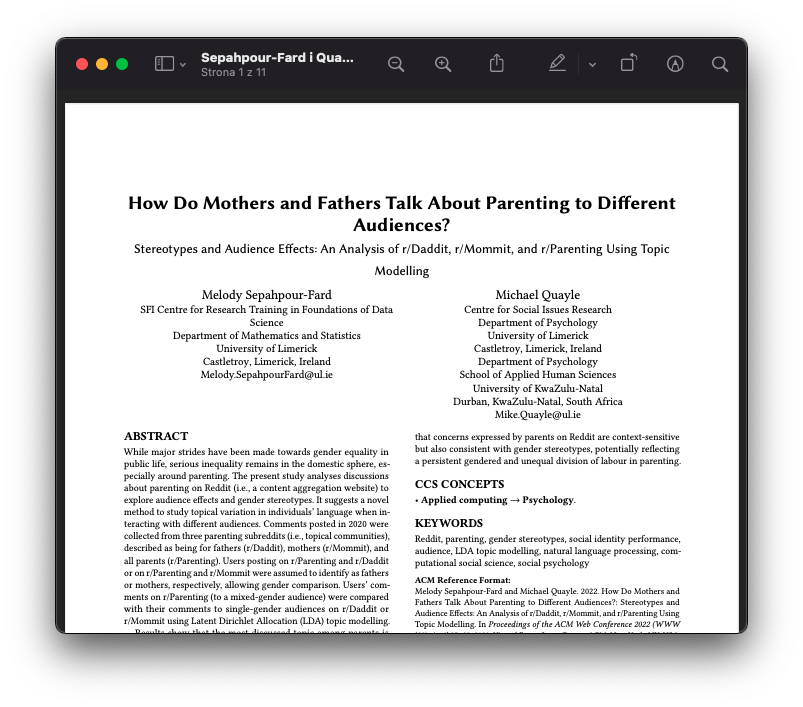
\includegraphics[width = \textwidth]{reddit2.png}
        \end{figure}
    }
    \only<+>{
        \framesubtitle{(Sepahpour-Fard et al., 2022)}
        \begin{figure}
            \centering
            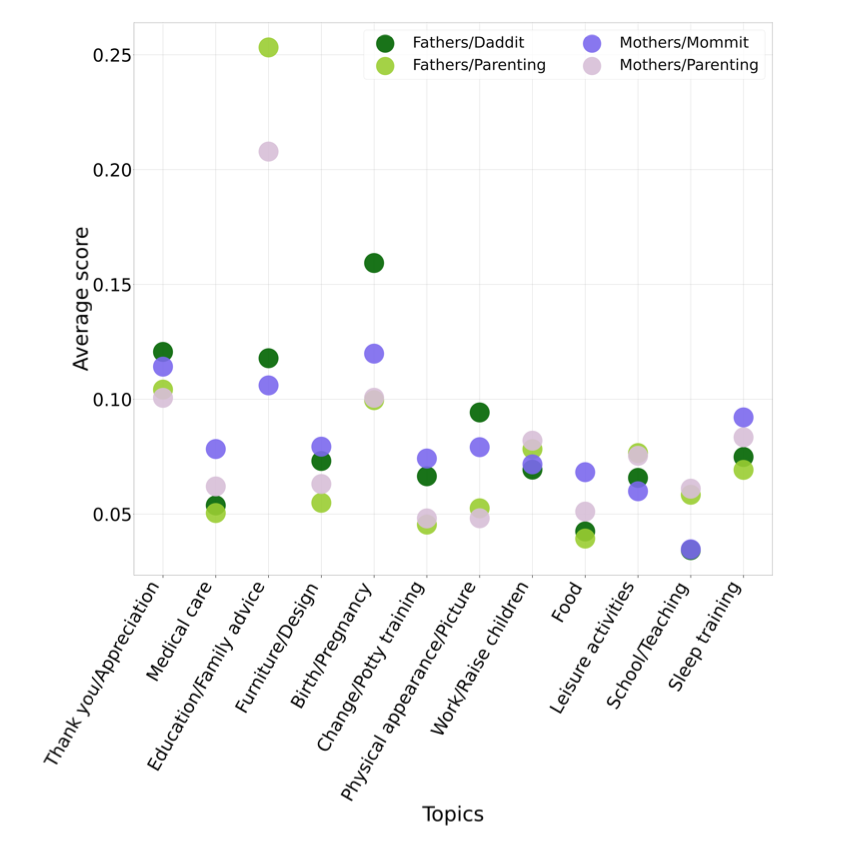
\includegraphics[width = .75\textwidth]{melody.png}
        \end{figure}
    }
    \only<+>{
        \begin{figure}
            \centering
            \includegraphics[width = \textwidth]{poster.png}
        \end{figure}
    }
\end{frame}

\begin{frame}
    \frametitle{Wikipedia}
    \only<+>{
        \begin{figure}
            \centering
            
\includegraphics[width = .3\textwidth]{wiki_logo.png}
        \end{figure}
    }
    \only<+>{
        \begin{figure}
            \centering
            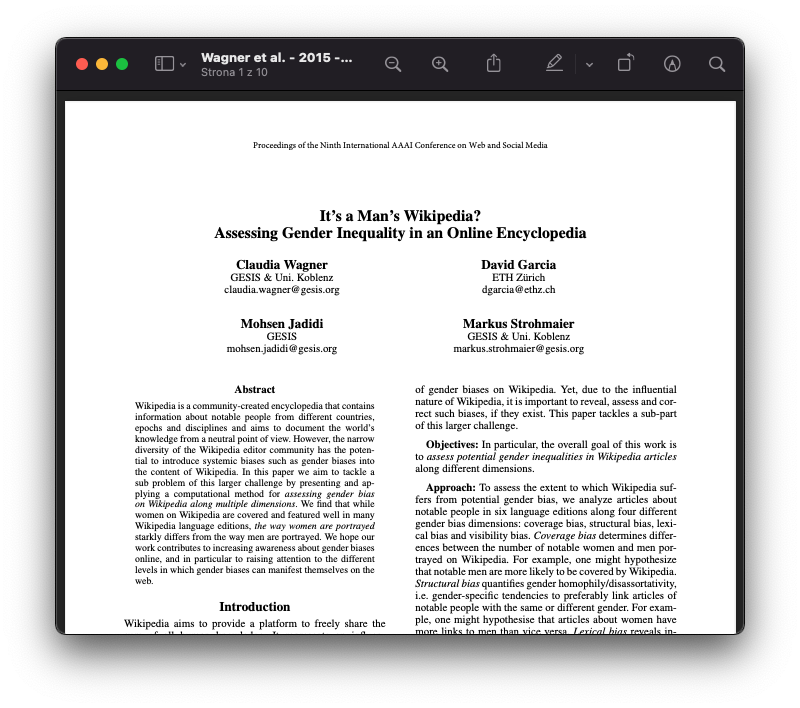
\includegraphics[width = \textwidth]{wiki1.png}
        \end{figure}
    }
    \only<+>{
        \framesubtitle{(Wagner et al., 2015)}
        \begin{itemize}
            \item \textbf{Coverage bias} determines differences between the
            number of notable women and men portrayed on Wikipedia.             
            \item \textbf{Visibility bias} reflects how many articles about men
            or women make it to the front page of Wikipedia.        
            \item \textbf{Structural bias} quantifies gender homophily/disassortativity,
            i.e. gender-specific tendencies to preferably link articles of
            notable people with the same or different gender. 
            \item \textbf{Lexical bias} reveals inequalities in the words used
            to describe notable men and women on Wikipedia.
        \end{itemize}
    }
    \only<+>{
        \framesubtitle{(Wagner et al., 2015)}
        \begin{itemize}
            \item \textbf{Coverage bias:} Men and women are covered equally well
            in all six Wikipedia language editions. 
            \item \textbf{Visibility bias:} No evidence for male-bias in the
            selection procedure of articles that are featured on the startpage
            of the English Wikipedia.
            \item \textbf{Structural bias:} Women on Wikipedia tend
            to be more linked to men than vice versa. 
            \item \textbf{Lexical bias:} Romantic relationships and
            family-related issues are much more frequently discussed on
            Wikipedia articles about women than men.
        \end{itemize}
    }
    \only<+>{
        \begin{figure}
            \centering
            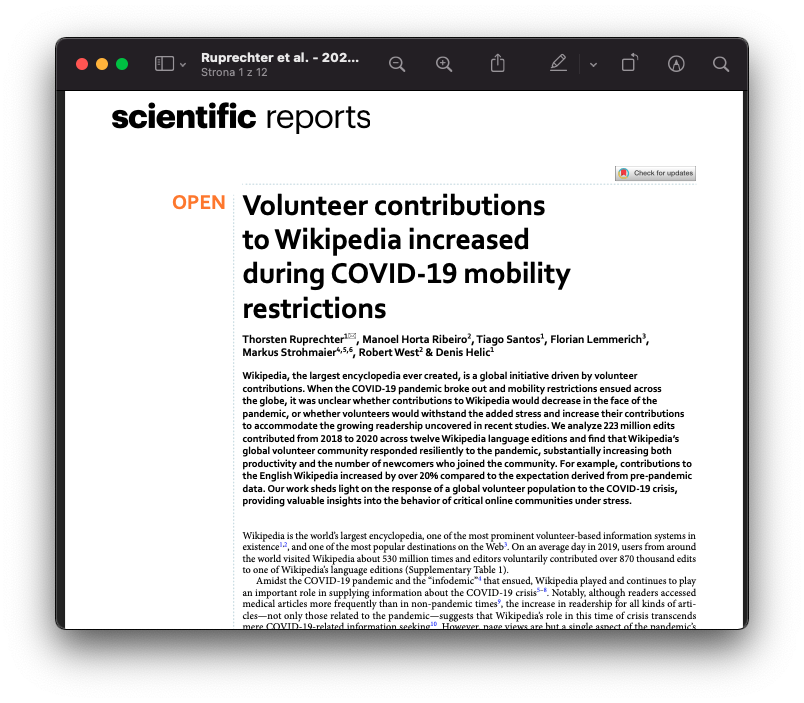
\includegraphics[width = \textwidth]{wiki2.png}
        \end{figure}
    }
    \only<+>{
        \framesubtitle{(Ruprechter et al., 2020)}
        \begin{figure}
            \centering
            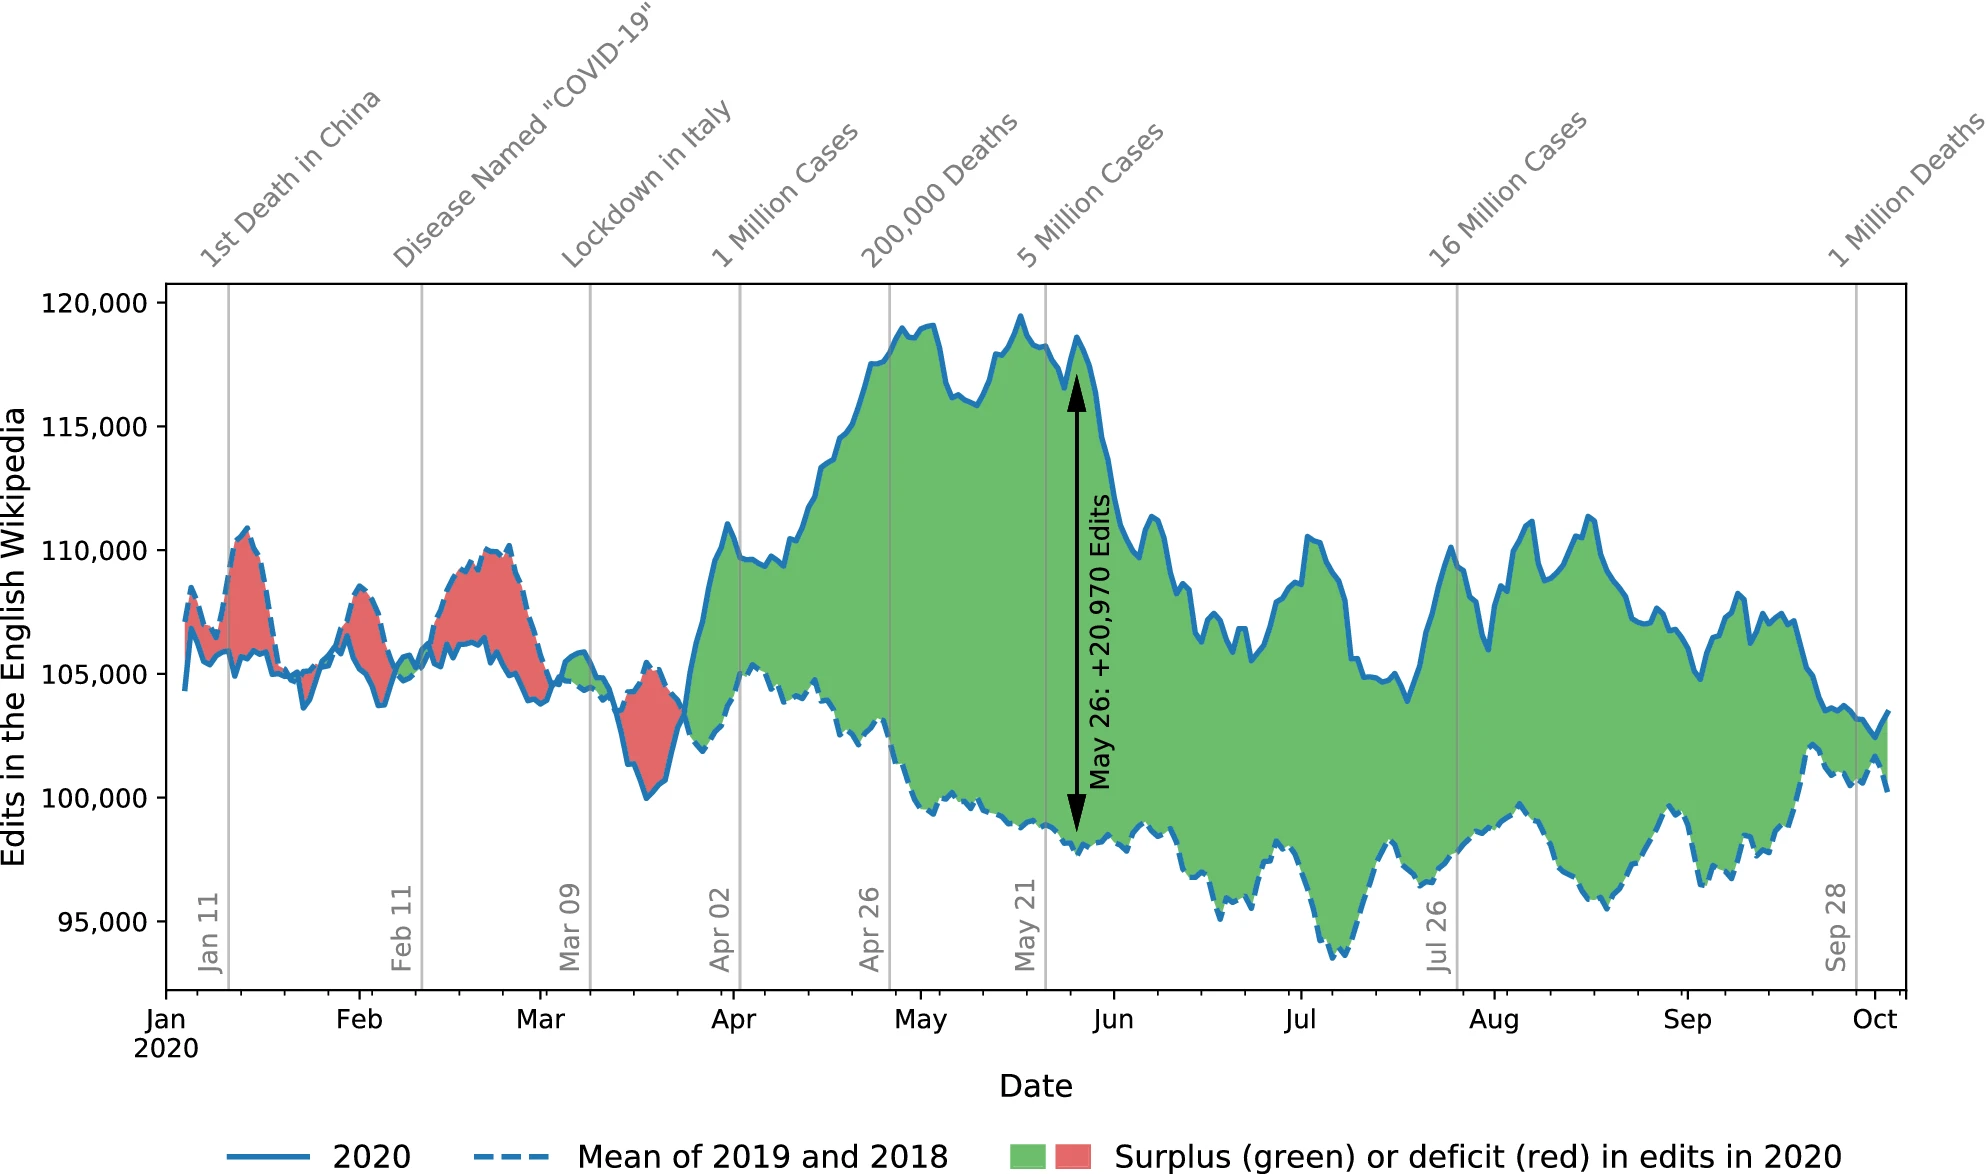
\includegraphics[width = \textwidth]{wikipedia_chart.png}
        \end{figure}
    }
\end{frame}

\begin{frame}
    \frametitle{The GDELT Project}
    \begin{tikzpicture}
        \node at (0,0) {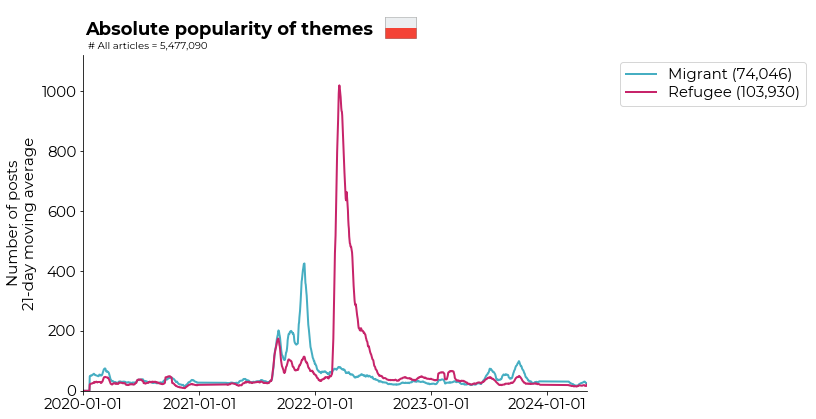
\includegraphics[width = 7cm]{pl_gdelt_themes_lines.png}};
        \node at (3.5,-3.75) {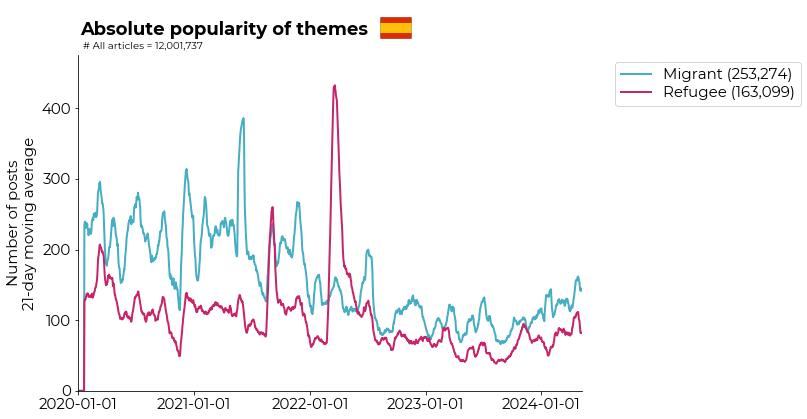
\includegraphics[width = 7cm]{esp_gdelt_themes_lines.png}};
    \end{tikzpicture}
\end{frame}

\section[API]{Web Application Programming Interface}

\begin{frame}
    \only<+>{
        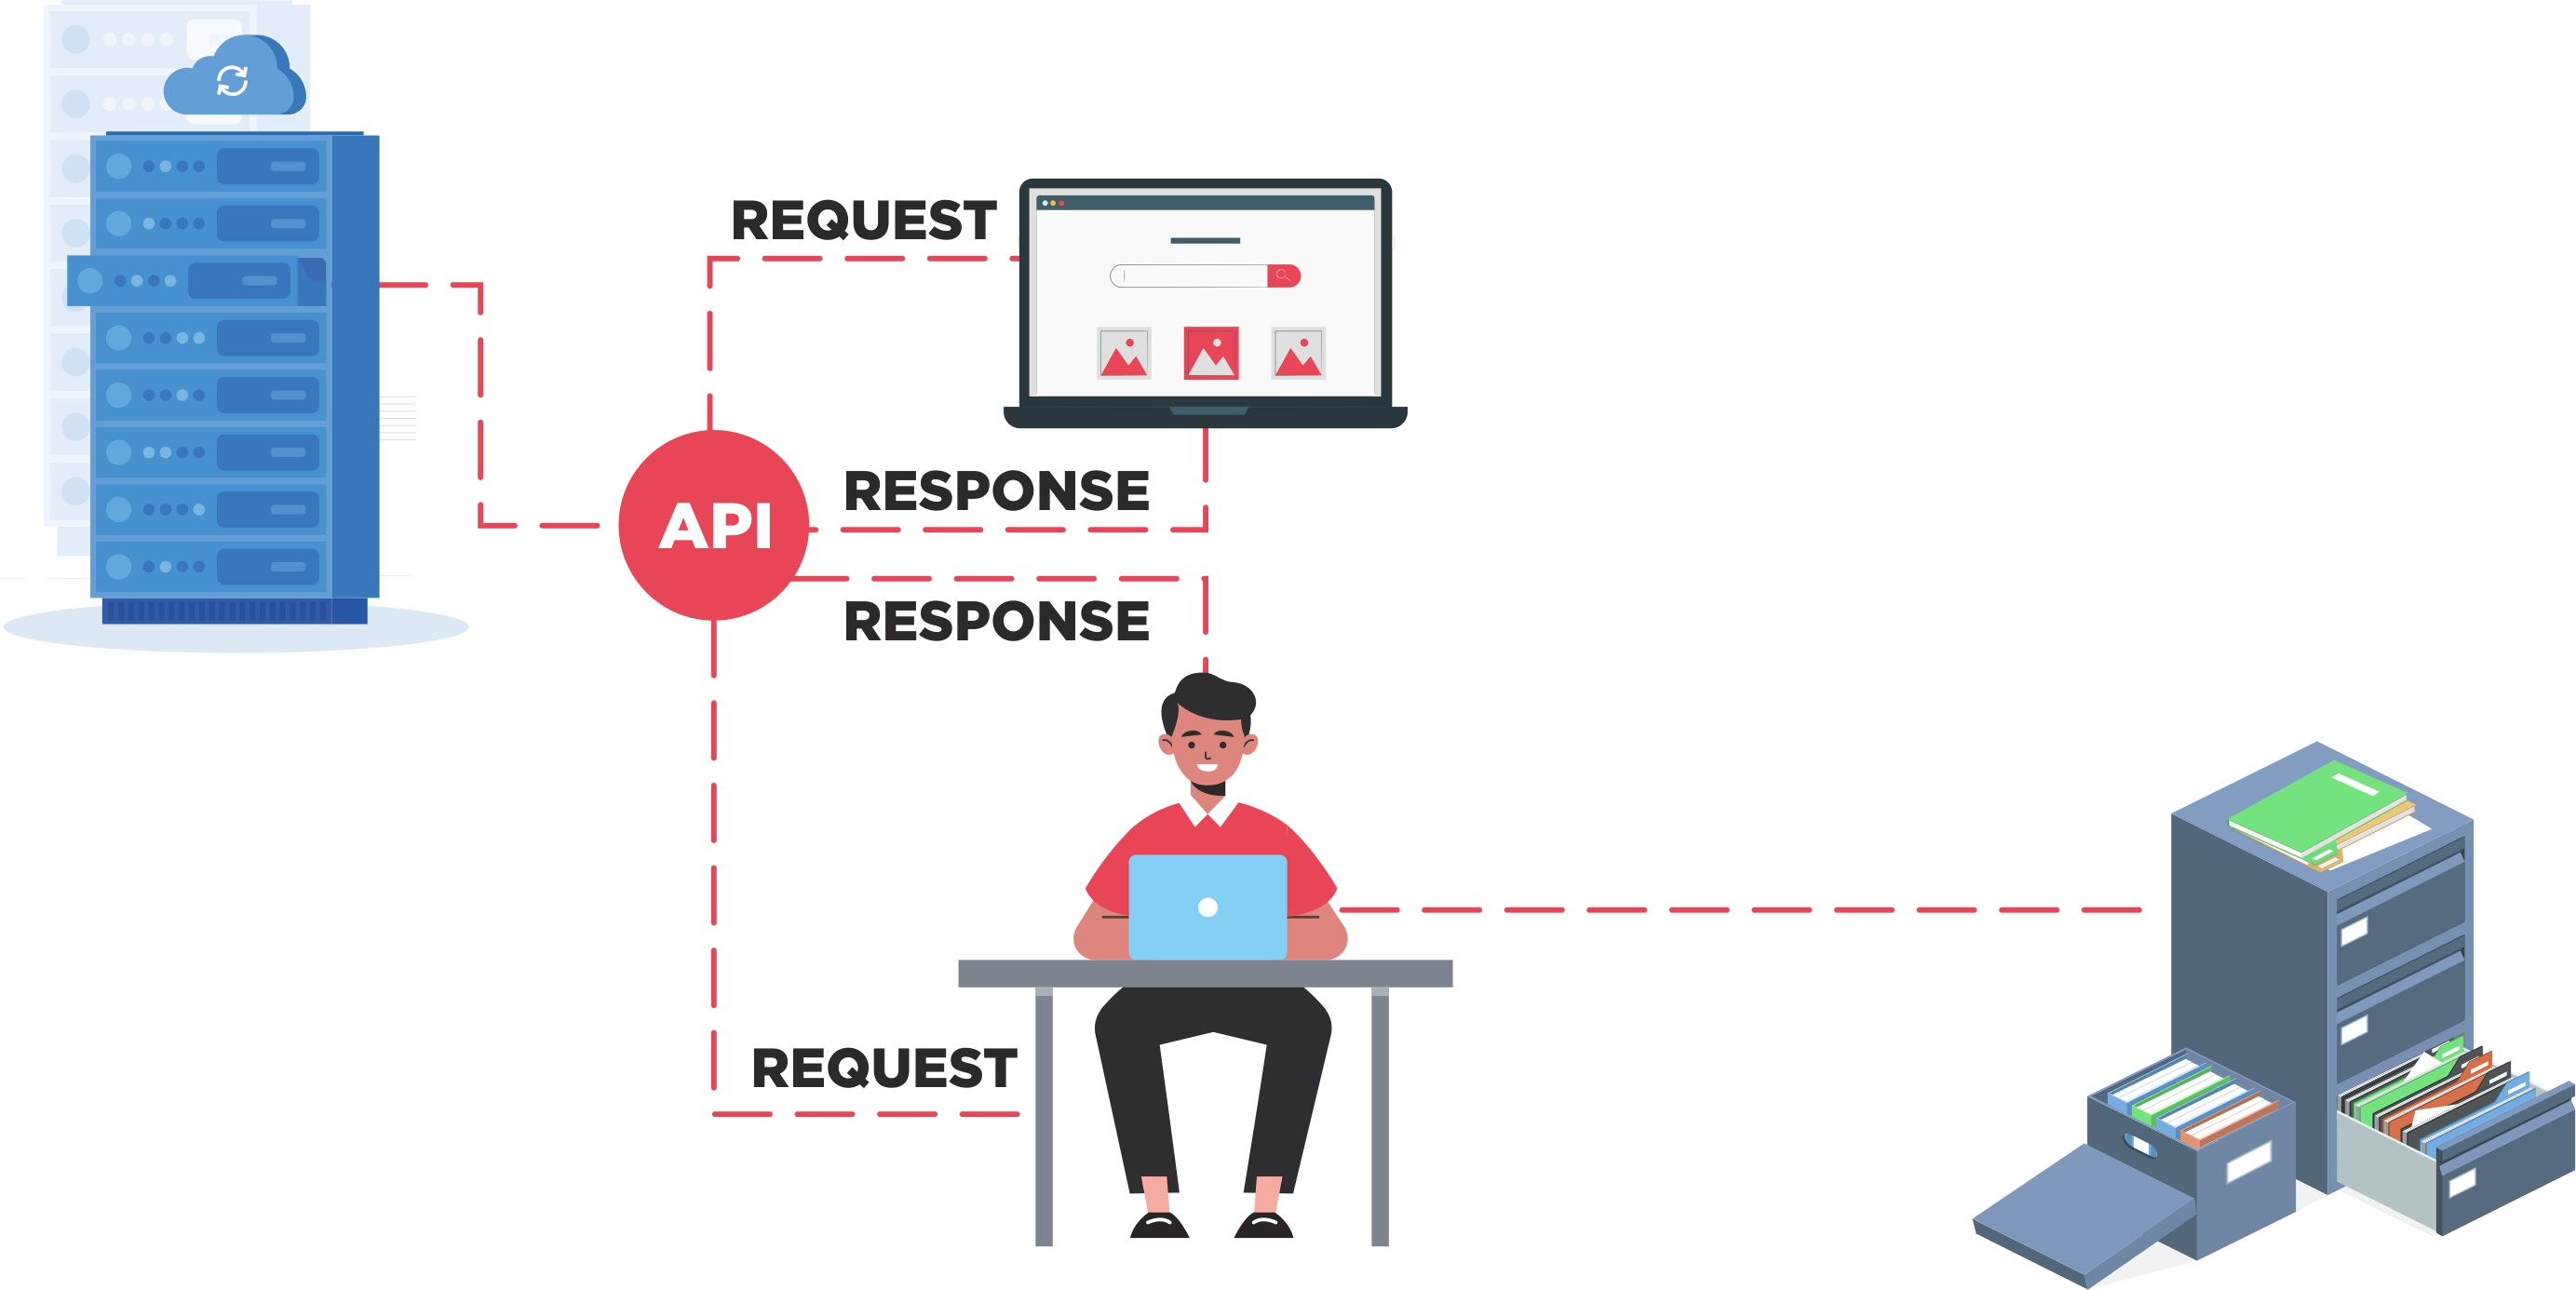
\includegraphics[width = \framewidth]{png/api.jpg}
    }
    \only<+>{
        \begin{definition}
            \emph{Aplication Programming Interface} is a communication protocol between a client and a server intended to simplify the building of client-side software. In other words, it is a contract between the client and the server which defines the format of possible requests and format of the response (i.e. format of the data).
        \end{definition}
    }
\end{frame}

%%  \subsection{HTML}
%%  \begin{frame}
%%      \only<+>{
%%          \frametitle{Web browsing}
%%          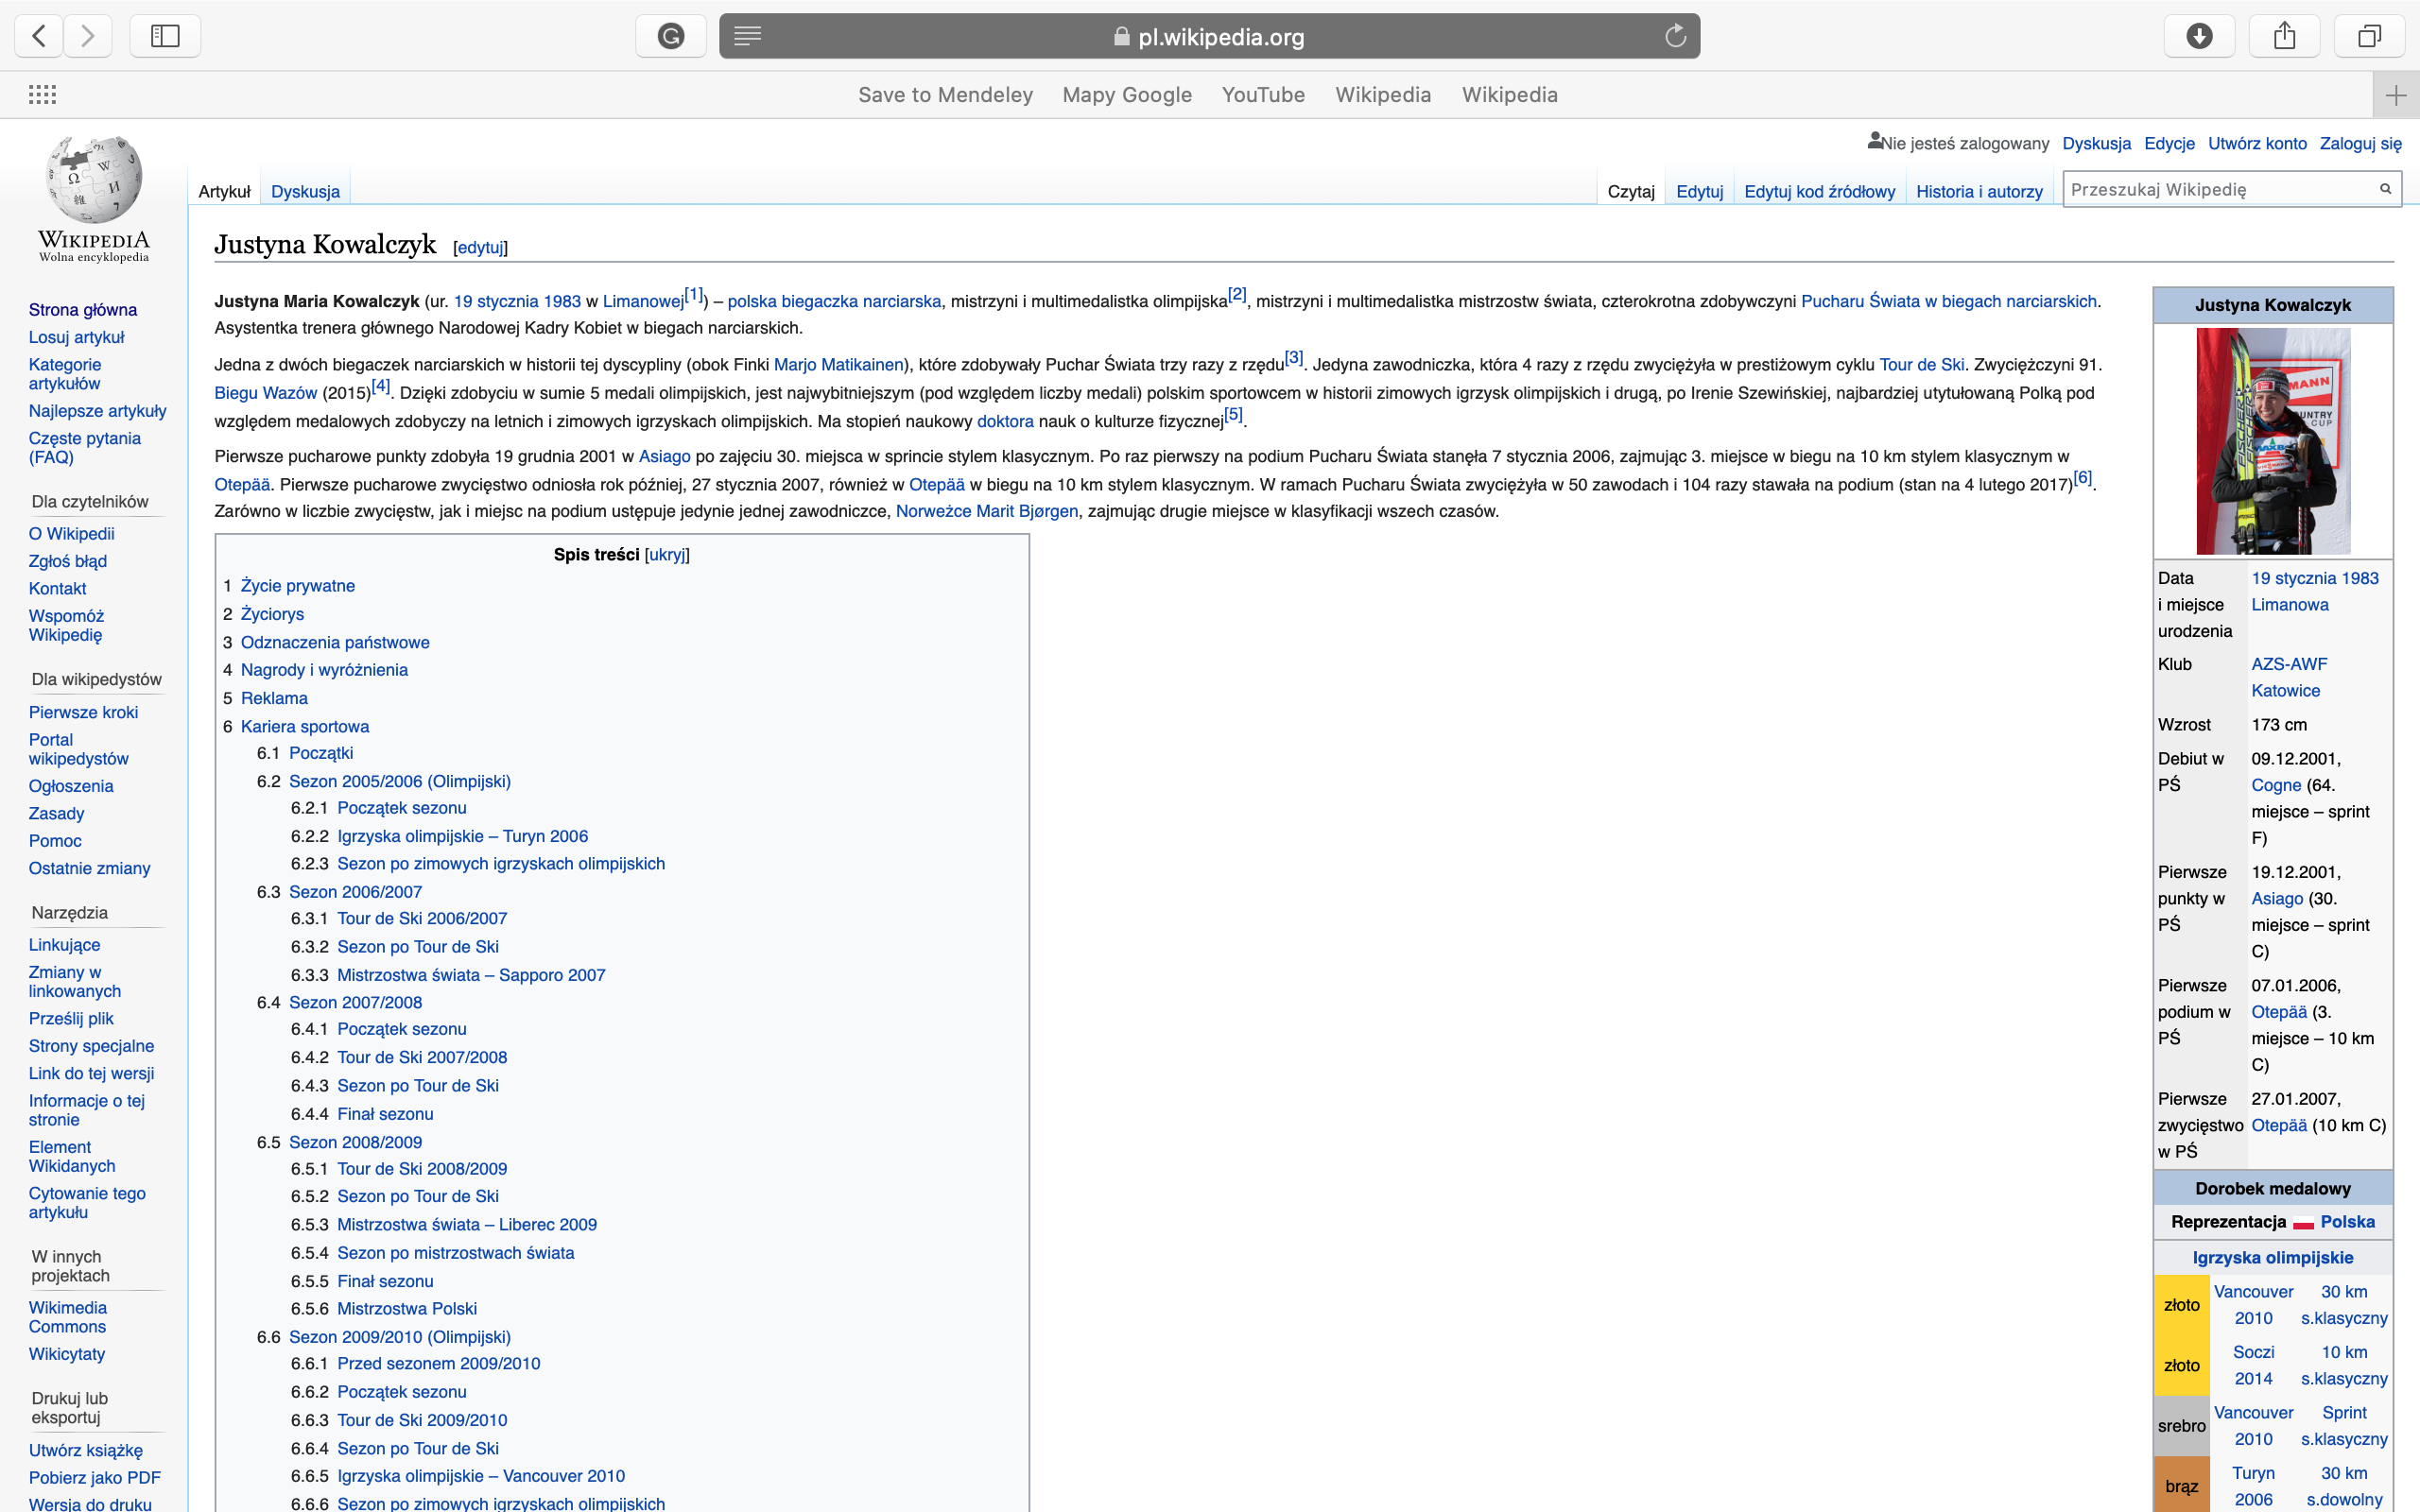
\includegraphics[width = \framewidth]{png/webpage.png}
%%      }
%%      \only<+>{
%%          \frametitle{Web browsing}
%%          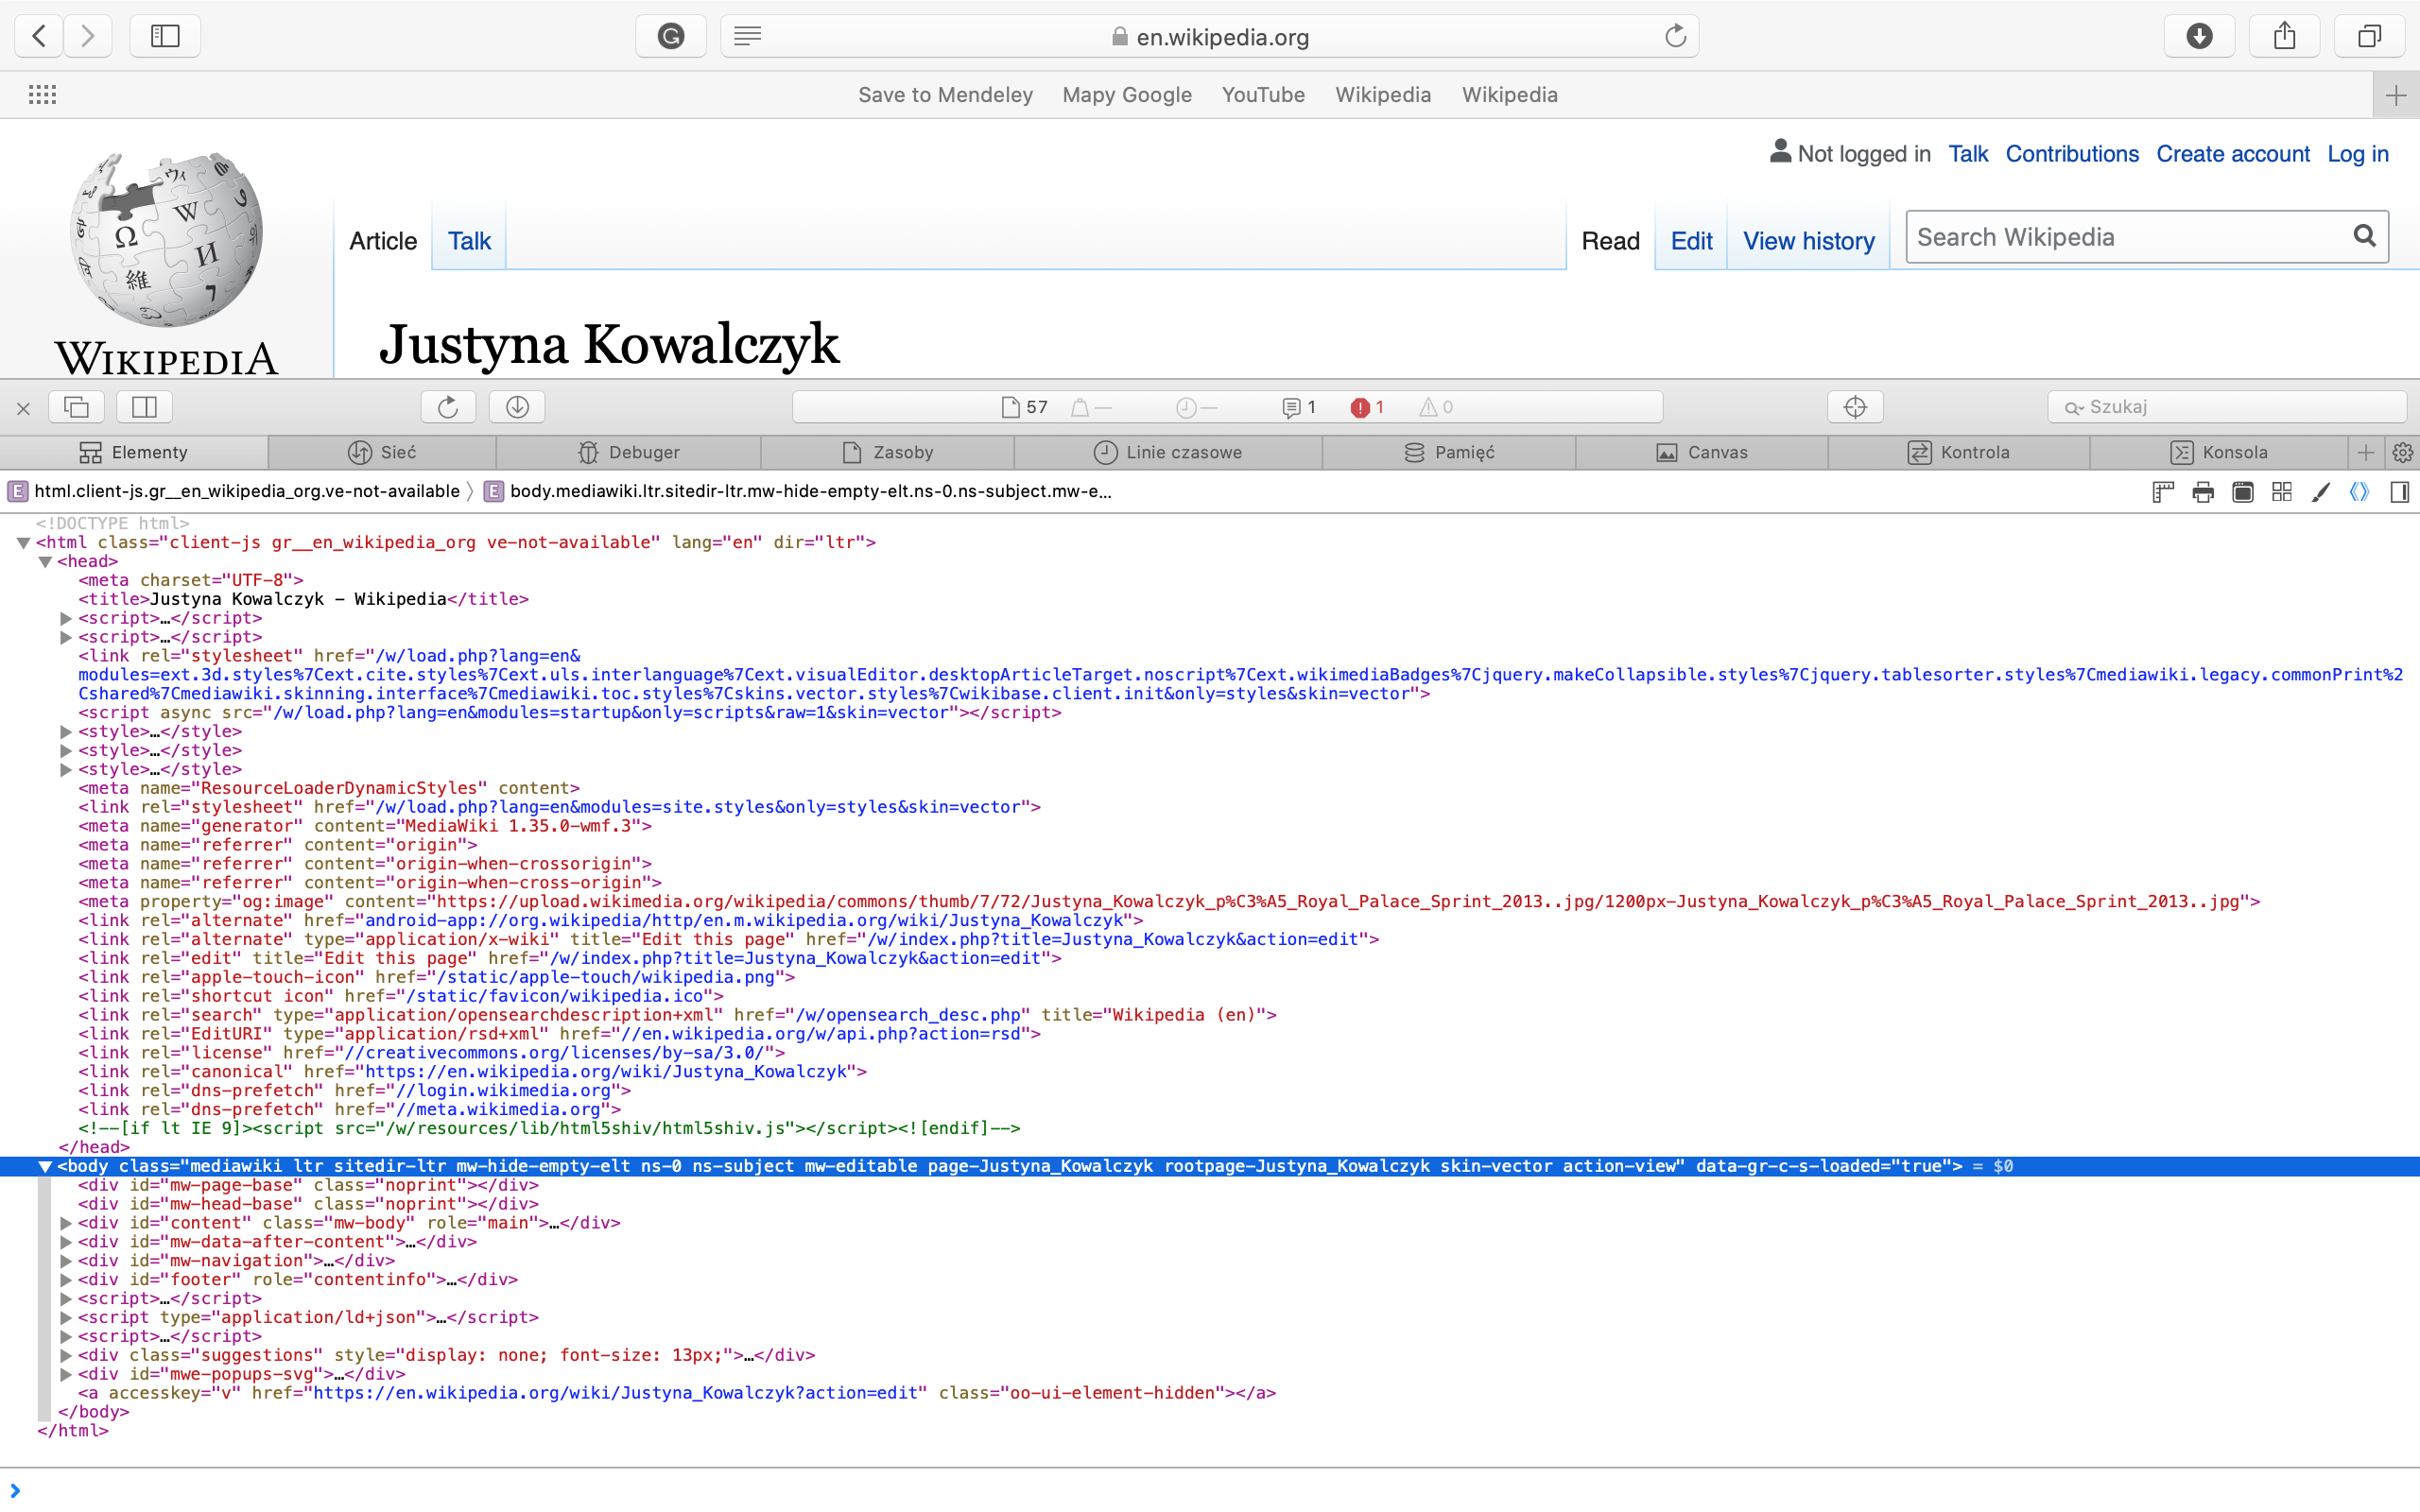
\includegraphics[width = \framewidth]{png/webpage_html.png}
%%      }
%%      \only<+>{
%%          \frametitle{Hypertext Markup Language}
%%          \begin{definition}
%%              \emph{Hypertext Markup Language} (HTML) is the standard markup language for documents designed to be displayed in a web browser. It can be assisted by technologies such as Cascading Style Sheets (CSS) and scripting languages such as JavaScript.
%%              Web browsers receive HTML documents from a web server or local storage and render the documents into multimedia web pages. HTML describes the structure of a web page semantically and originally included cues for the appearance of the document.
%%          \end{definition}
%%      }
%%  \end{frame}
%%  
%%  \begin{frame}[fragile]
%%      \frametitle{HTML example}
%%      \begin{minted}[escapeinside=||,mathescape=true]{html}
%%  <!DOCTYPE html>
%%  <html>
%%      <head>
%%          <title>
%%              Justyna Kowalczyk fandom
%%          </title>
%%      </head>
%%      <body>
%%          <p>
%%              Justyna Kowalczyk |<|3
%%          </p>
%%      </body>
%%  </html>
%%      \end{minted}
%%  \end{frame}
%%  
%%  \subsection{CSS}
%%  
%%  \begin{frame}
%%          \frametitle{Cascading Style Sheets}
%%          \begin{definition}
%%              \emph{Cascading Style Sheets} (CSS) is a style sheet language used for describing the presentation of a document written in a markup language like HTML.
%%          \end{definition}
%%  \end{frame}
%%  
%%  \begin{frame}[fragile]
%%      \frametitle{CSS}
%%      \begin{minted}[escapeinside=||,mathescape=true]{html}
%%  <!DOCTYPE html>
%%  <html>
%%      <head>
%%          <title>
%%              Justyna Kowalczyk fandom
%%          </title>
%%          <style>
%%              .person {
%%                  color: red;
%%              }
%%          </style>
%%      </head>
%%      <body>
%%          <p class="person">
%%              Justyna Kowalczyk |<|3
%%          </p>
%%      </body>
%%  </html>
%%      \end{minted}
%%  \end{frame}
%%  
%%  \begin{frame}
%%      \only<+>{
%%          \frametitle{Web browsing without CSS}
%%          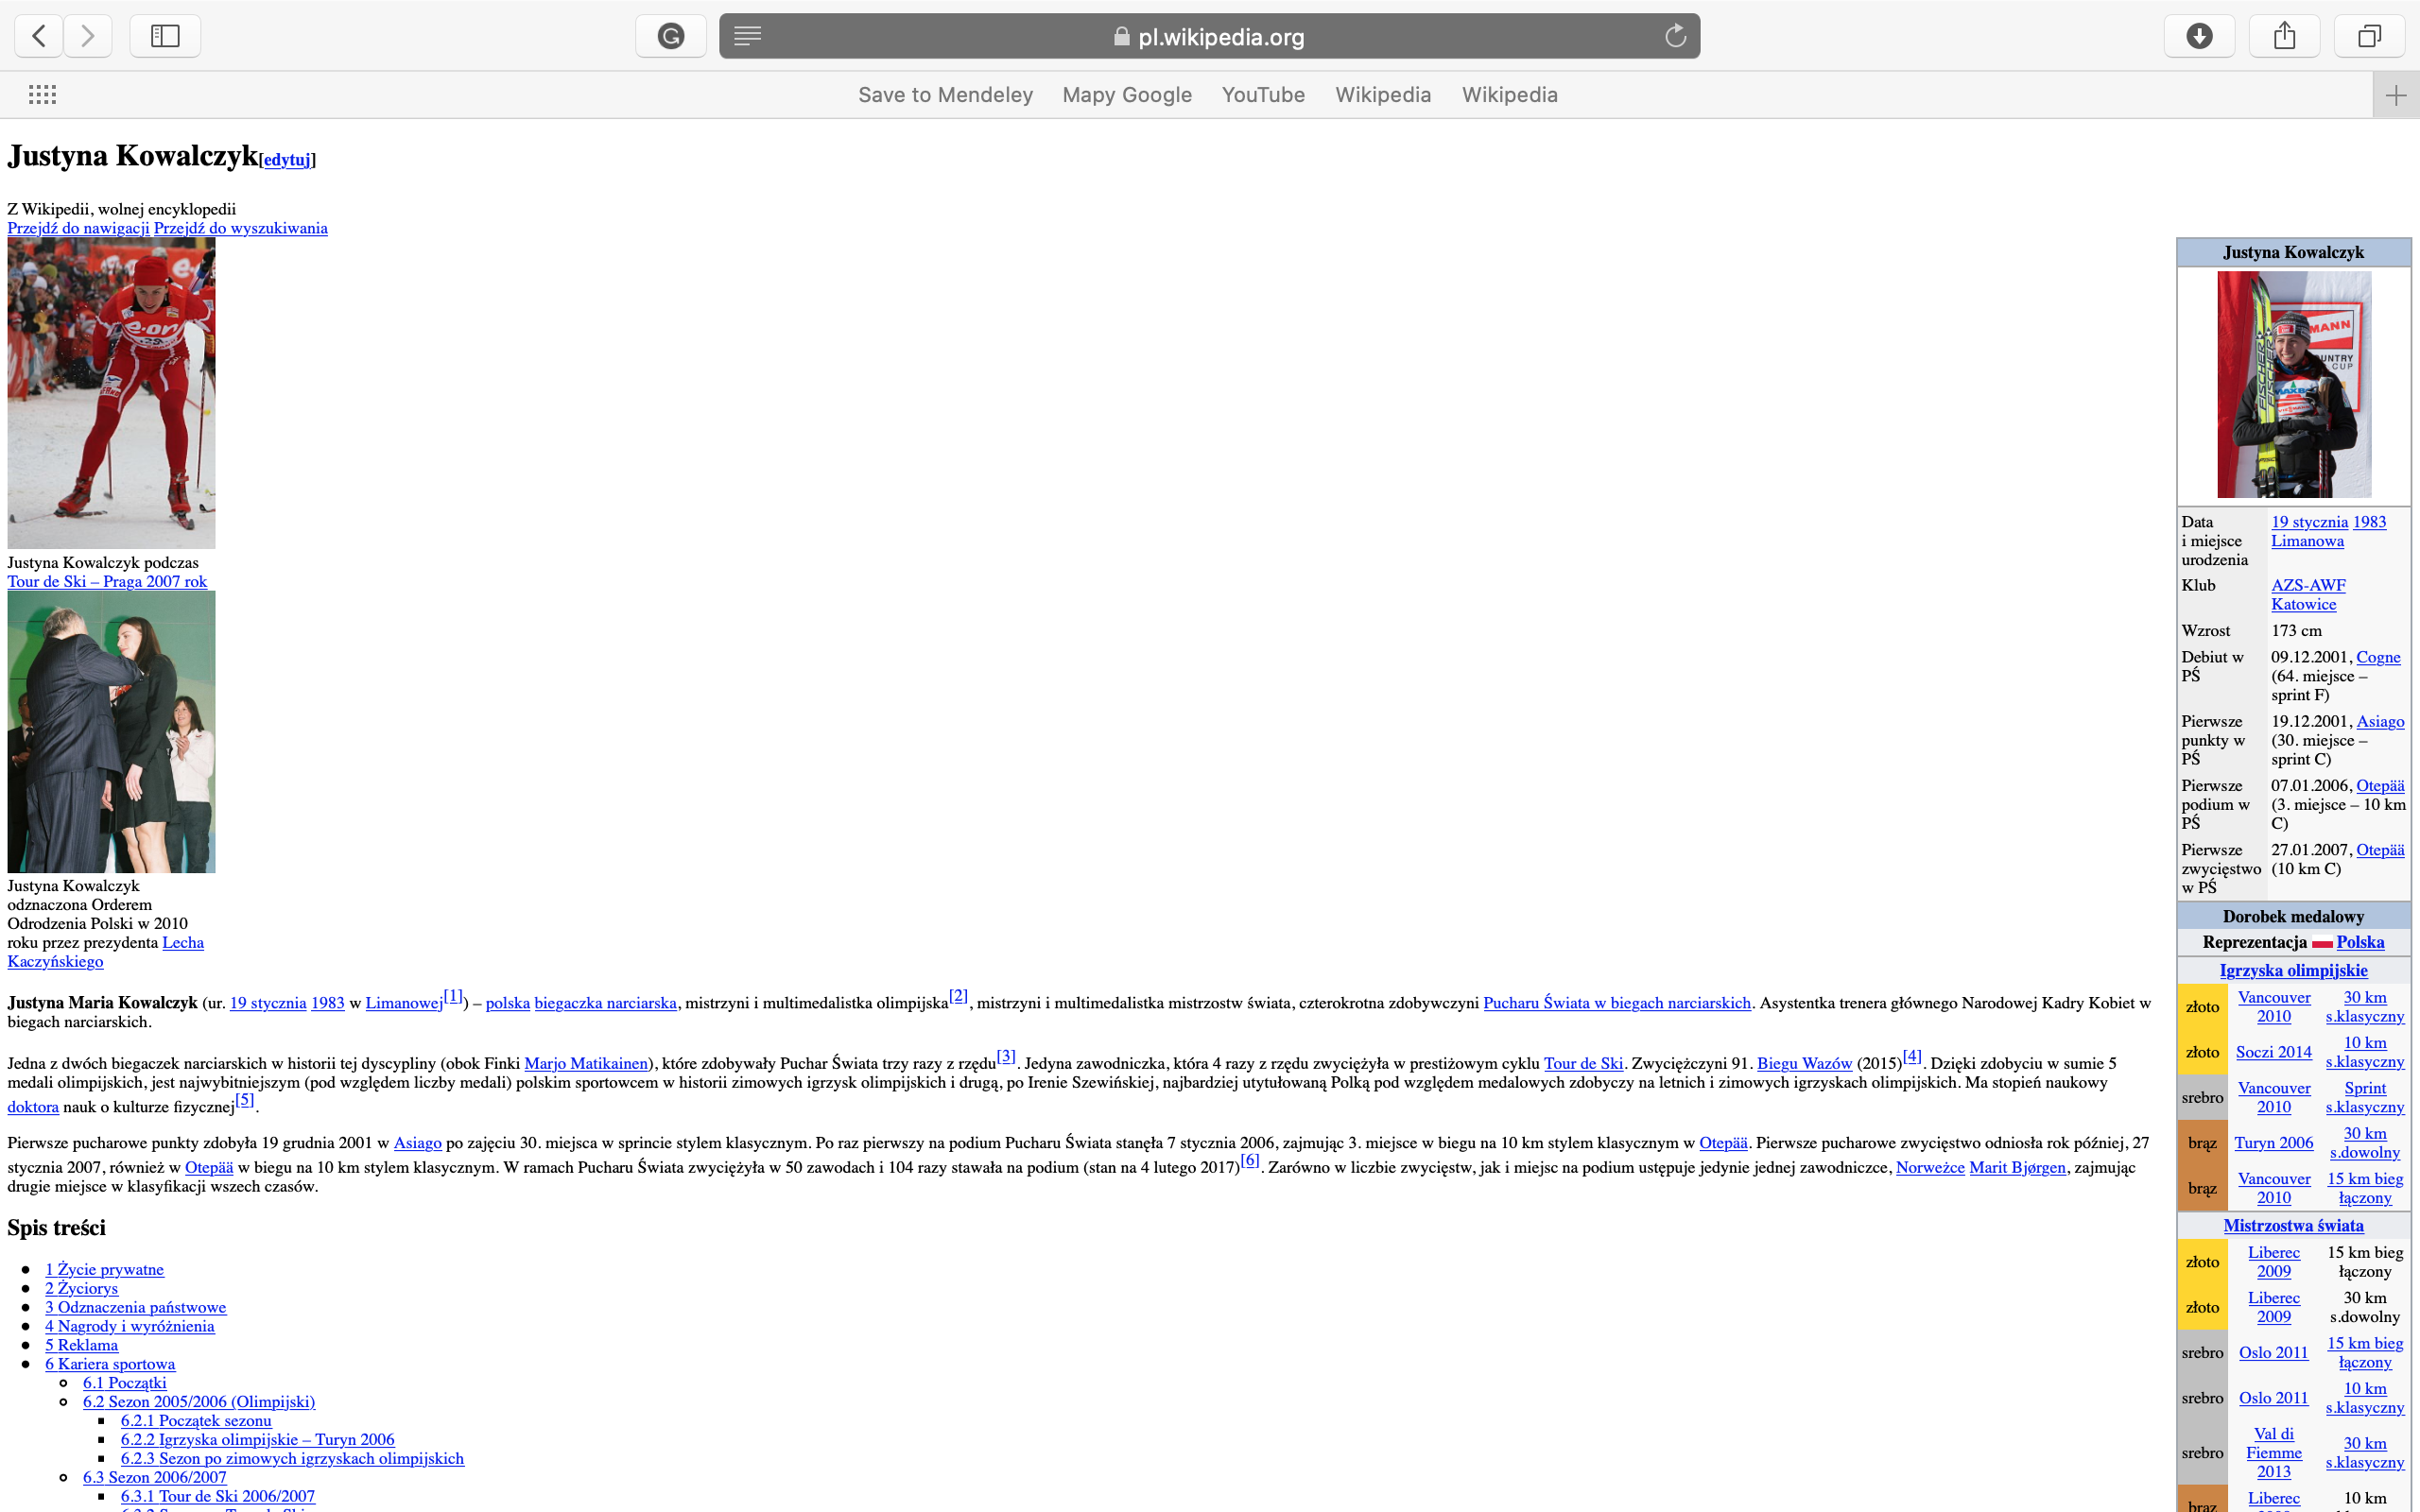
\includegraphics[width = \framewidth]{png/webpage_nostyle.png}
%%      }
%%      \only<+>{
%%          \frametitle{Web browsing without CSS}
%%          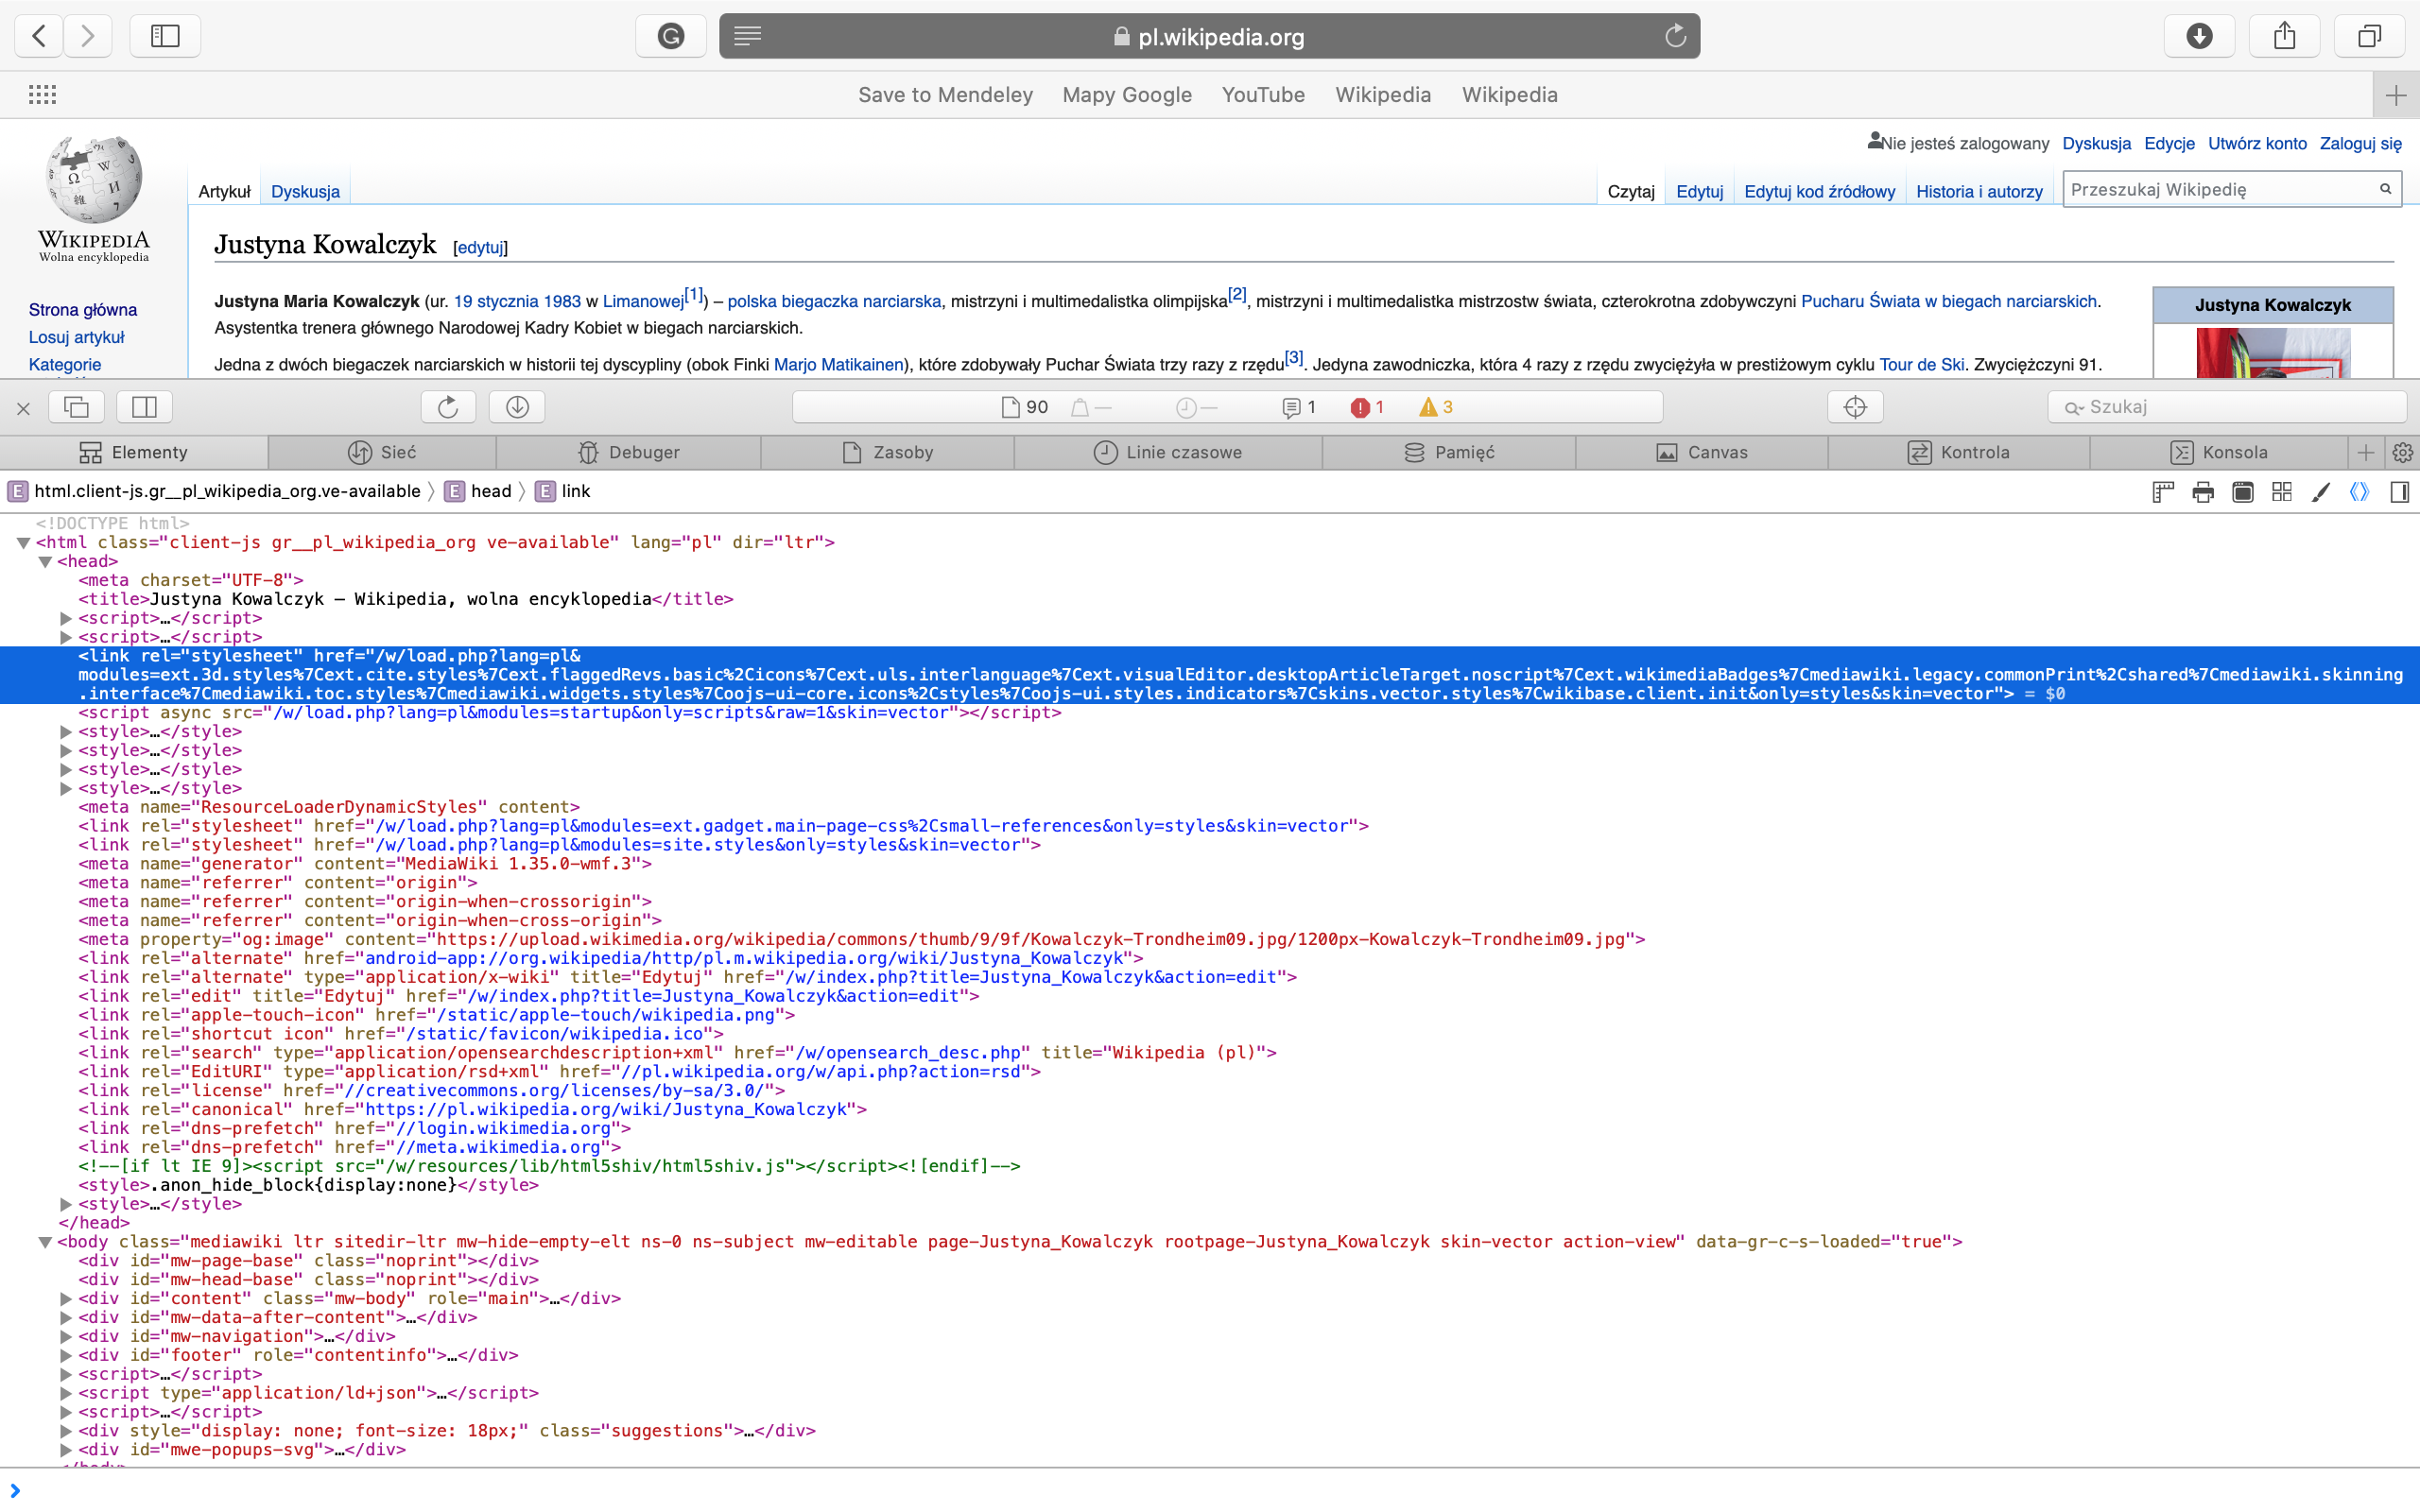
\includegraphics[width = \framewidth]{png/webpage_css.png}
%%      }
%%  \end{frame}

\begin{frame}
    \only<+>{
        \frametitle{Types of Web APIs}
        \setbeamercovered{transparent}
        \begin{itemize}
            \item<0> SOAP (Simple Object Access Protocol)
            \item<0> RPC (Remote Procedure Call)
            \item REST (REpresentational State Transfer)
        \end{itemize}
    }
\end{frame}
\subsection{REST}
\begin{frame}
    \only<1>{
        \frametitle{REST (REpresentational State Transfer)}
        \begin{definition}
            The \emph{Representational State Transfer} (REST) is an abstraction of the architectural elements within a distributed hypermedia system. It ignores the details of component implementation and protocol syntax to focus on the roles of components, the constraints upon their interaction with other components, and their interpretation of significant data elements. It encompasses the fundamental constraints upon components, connectors, and data that define the basis of the Web architecture, and thus the essence of its behavior as a network-based application.
        \end{definition}
    }
    \only<2,4,6,8,13,15>{
        \frametitle{REST constraints}
        \begin{enumerate}
            \item<2-> Client-Server
            \item<4-> Stateless
            \item<6-> Cache
            \item<8-> Uniform Interface
            \item<13-> Layered System
            \item<15-> Code-On-Demand*
        \end{enumerate}
    }
    \only<3>{
        \frametitle{Clinet-Server}
        Client and Server are \alert{independent}. They must be able to evolve separately without any dependency on each other. In other words, the application (client) should work regardless of changes on the server-side and the other way around.
    }
    \only<5>{
        \frametitle{Stateless}
        Each request sent by the client to the server must contain \alert{all of the information necessary to understand the request}, and cannot take advantage of any stored context on the server.
    }
    \only<7>{
        \frametitle{Cache}
        Cache constraints require that the data within a response to a request be implicitly or explicitly labeled as cacheable or non-cacheable. If a response is cacheable, then \alert{a client cache is given the right to reuse that response data for later}, equivalent requests.
    }
    \only<9-12>{
        \frametitle{Uniform Interface}
        \begin{enumerate}
            \item<9-> Resource-Based \only<9>{-- The resources themselves are conceptually separate from the representations that are returned to the client. For example, \alert<9>{the server does not send its database}, but rather, some HTML, XML or JSON that represents some database records expressed.}
            \item<10-> Manipulation of Resources Through Representations \only<10>{-- When a client \alert<10>{holds a representation of a resource}, including any metadata attached, it \alert<10>{has enough information to modify or delete the resource on the server}, provided it has permission to do so.}
            \item<11-> Self-descriptive Messages \only<11>{-- Each message includes \alert<11>{enough information to describe how to process the message}. For example, which parser to invoke. Responses also explicitly indicate their cache-ability.}
            \item<12-> Hypermedia as the Engine of Application State (HATEOAS) \only<12>{-- Clients deliver state via \alert<12>{body contents, query-string parameters, request headers and the requested universal resource identifier} (the resource name). Services deliver the state to clients via \alert<12>{body content, response codes, and response headers}. This is technically referred to as hypermedia (or hyperlinks within hypertext).}
        \end{enumerate}
    }
    \only<14>{
        \frametitle{Layered System}
        A client cannot ordinarily \alert{tell whether it is connected directly to the end server} or an intermediary along the way. Intermediary servers may improve system scalability by enabling load-balancing and by providing shared caches. Layers may also enforce security policies.
    }
    \only<16>{
        \frametitle{Code-On-Demand*}
        Servers are able to send \alert{executable code} to support part of the application on the client-side. In other words, most of the time the server sends a representation of the resources in the form of JSON or XML, but it can also send an executable code.
    }
\end{frame}

\subsection{HTTP}
\begin{frame}
    \only<+>{
        \frametitle{Hypertext Transfer Protocol}
        \begin{definition}
            \emph{Hypertext Transfer Protocol} (HTTP) is a protocol that allows the fetching of resources, such as HTML documents. It is the foundation of any data exchange on the Web and it is a client-server protocol, which means requests are initiated by the recipient, usually the Web browser. A complete document is reconstructed from the different sub-documents fetched, for instance, text, layout description, images, videos, scripts, and more.
        \end{definition}
    }
    \only<+>{
        \frametitle{HTTP Requests}
        HTTP Requests is typically composed of:
        \begin{itemize}
            \item A start-line (HTTP method, URL/URI, and HTTP version).
            \item An optional set of HTTP headers specifying the request, or describing the body included in the message.
            \item An optional body containing data associated with the request.
        \end{itemize}

    }
    \only<+>{
        \frametitle{HTTP Request Methods}
        \begin{itemize}
            \item GET -- requests a representation of the specified resource
            \item POST -- is used to submit an entity to the specified resource, often causing a change in state or side effects on the server.
            \item PUT -- replaces all current representations of the target resource with the request payload.
            \item DELETE -- deletes the specified resource.
            \item PATCH -- is used to apply partial modifications to a resource.
        \end{itemize}
        %\footnote{Detailed documentation on \textcolor{blue}{\href{https://developer.mozilla.org/en-US/docs/Web/HTTP/Methods}{Request Methods}}}
    }
\end{frame}

\begin{frame}[fragile]
    \frametitle{HTTP Request}
    \begin{minted}{html}
    GET page/summary/Justyna_Kowalczyk HTTP/1.1
    Host: www.en.mikopedia.org/api/rest_v1/
    Accept: application/json
    User-Agent: m.biesaga@uw.edu.pl
    Body: {}
    \end{minted}
\end{frame}


\begin{frame}
    \only<+>{
        \frametitle{HTTP Response}
        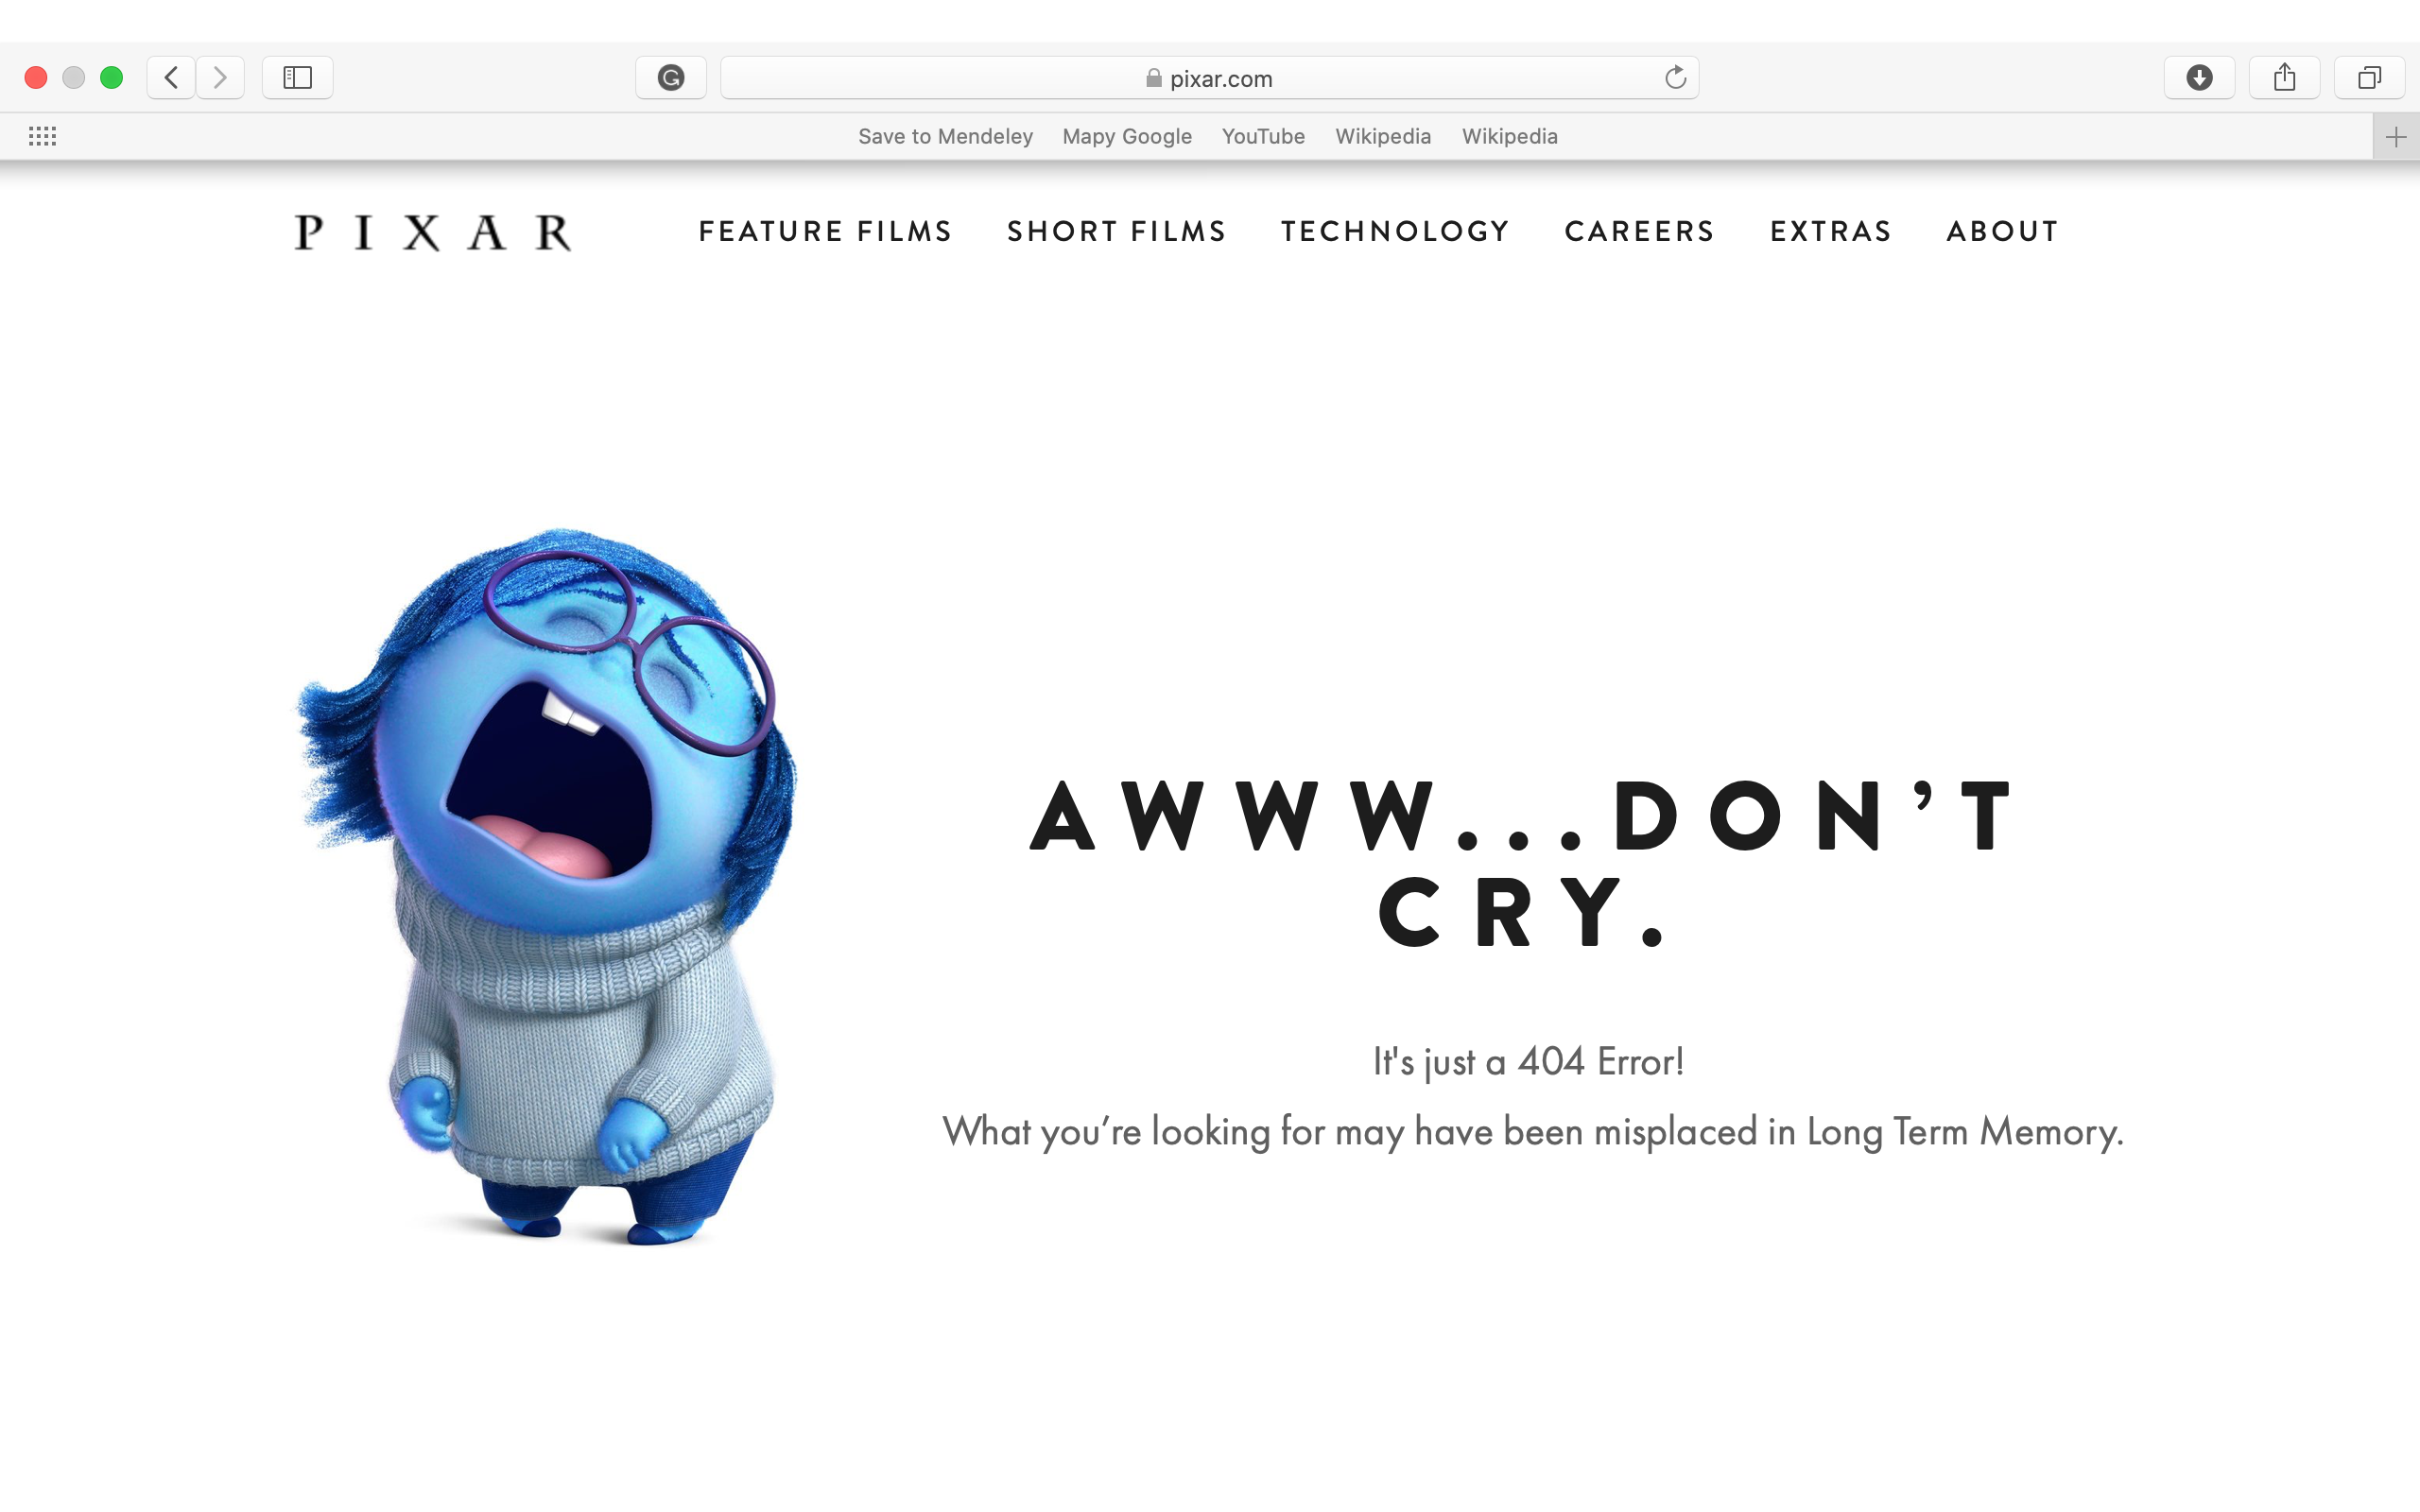
\includegraphics[width = \framewidth]{png/error_404.png}
    }
    \only<+>{
        \frametitle{HTTP Response}
        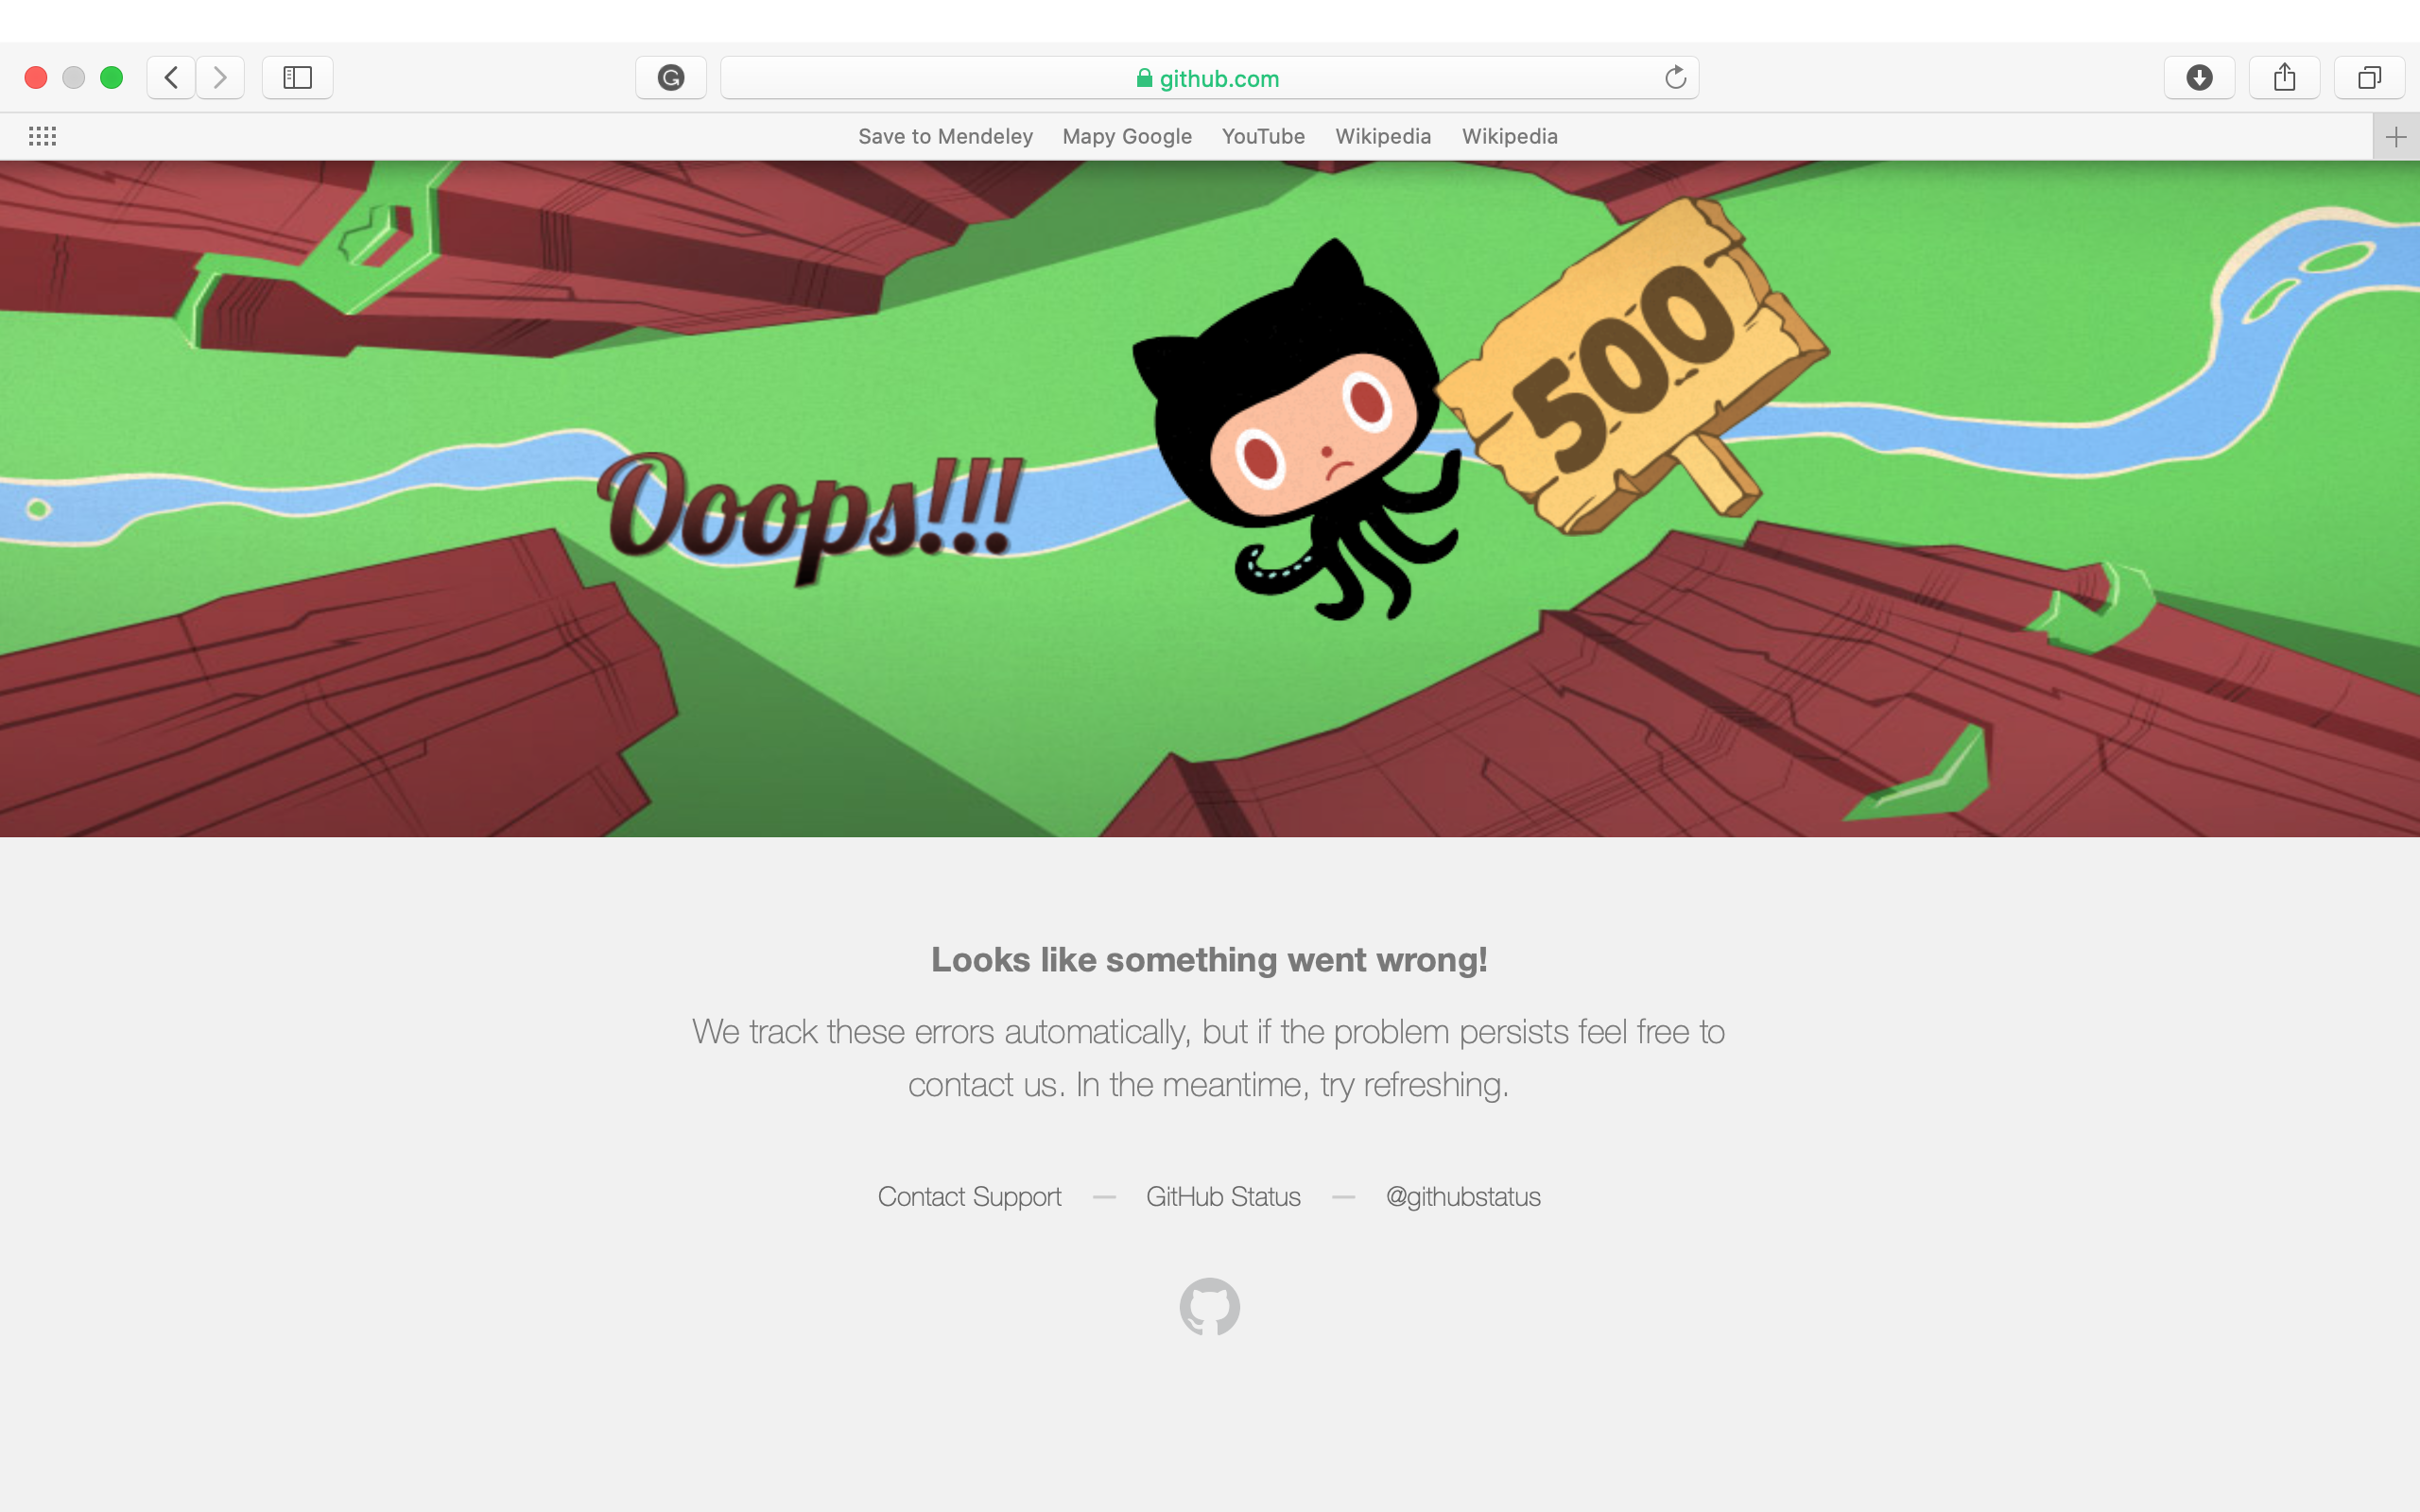
\includegraphics[width = \framewidth]{png/error_500.png}
    }
    \only<+>{
        \frametitle{HTTP Responses}
        HTTP Response is typically composed of:
        \begin{itemize}
            \item A status line (HTTP version, a status code, and a status text)
            \item A set of HTTP headers specifying the response, or describing the body included in the message.
            \item An optional body containing data associated with the response
        \end{itemize}
    }
    \only<+>{
        \frametitle{HTTP Response Status Codes}
        \begin{itemize}
            \item Informational response (100–199);
            \item Successful responses (200–299);
            \item Redirects (300–399);
            \item Client errors (400–499);
            \item Server errors (500–599).
        \end{itemize}
        %\footnote{Detailed documentation on \textcolor{blue}{\href{https://developer.mozilla.org/en-US/docs/Web/HTTP/Status}{Response Status Codes}}}
    }
\end{frame}

\begin{frame}[fragile]
    \frametitle{HTTP Response}
    \begin{minted}[escapeinside=||,mathescape=true]{html}
    HTTP/1.1 200 OK
    Access-control-allow-methods: GET,HEAD
    Age: 94618
    Content-language: en
    Content-length: 881
    Content-type: application/json
    Date: Wed, 30 Oct 2019 00:18:58 GMT
    Body: {
        "type": "standard",
        "title": "Justyna Kowalczyk",
        "page_id": 4212731,
        "lang": "en",
        "revision": revision,
        "summary": "Justyna Kowalczyk |<|3"
    }
    \end{minted}
\end{frame}

\begin{frame}
    \frametitle{Bibliography}
    \tiny
    \begin{enumerate}
        %% \item Colleoni, E., Rozza, A., \& Arvidsson, A. (2014). Echo Chamber or Public Sphere? Predicting Political Orientation and Measuring Political Homophily in Twitter Using Big Data: Political Homophily on Twitter. Journal of Communication, 64(2), 317–332. \href{https://doi.org/10.1111/jcom.12084}{\textcolor{blue}{https://doi.org/10.1111/jcom.12084}}
        %% \item Ozalp, S., Williams, M. L., Burnap, P., Liu, H., \& Mostafa, M. (2020). Antisemitism on Twitter: Collective Efficacy and the Role of Community Organisations in Challenging Online Hate Speech. Social Media + Society, 6(2), 205630512091685. \href{https://doi.org/10.1177/2056305120916850}{\textcolor{blue}{https://doi.org/10.1177/2056305120916850}}
        %% \item Mancini, A., Desiderio, A., Di Clemente, R., \& Cimini, G. (2022). Self-induced consensus of Reddit users to characterise the GameStop short squeeze. Scientific Reports, 12(1), 13780. \href{https://doi.org/10.1038/s41598-022-17925-2}{\textcolor{blue}{https://doi.org/10.1038/s41598-022-17925-2}}
        \item Sepahpour-Fard, M., \& Quayle, M. (2022). How Do Mothers and Fathers Talk About Parenting to Different Audiences?: Stereotypes and Audience Effects: An Analysis of r/Daddit, r/Mommit, and r/Parenting Using Topic Modelling. Proceedings of the ACM Web Conference 2022, 2696–2706. \href{https://doi.org/10.1145/3485447.3512138}{\textcolor{blue}{https://doi.org/10.1145/3485447.3512138}}
        \item Wagner, C., Garcia, D., Jadidi, M., \& Strohmaier, M. (2015). It’s a Man’s Wikipedia? Assessing Gender Inequality in an Online Encyclopedia. Proceedings of the ninth International AAAI Conference of Web and Social Media, 9, 454–463. \href{https://ojs.aaai.org/index.php/ICWSM/article/view/14628}{\textcolor{blue}{https://ojs.aaai.org/index.php/ICWSM/article/view/14628}}
        \item Ruprechter, T., Horta Ribeiro, M., Santos, T., Lemmerich, F., Strohmaier, M., West, R., \& Helic, D. (2021). Volunteer contributions to Wikipedia increased during COVID-19 mobility restrictions. Scientific Reports, 11(1), 21505. \href{https://doi.org/10.1038/s41598-021-00789-3}{\textcolor{blue}{https://doi.org/10.1038/s41598-021-00789-3}}
    \end{enumerate}
    
\end{frame}



\end{document}
